\chapter{绪论}\label{chap:intro}



\section{概述}

自1995年实验中首次在冷原子系统中观测到玻色-爱因斯坦凝聚\cite{anderson1995observation,davis1995bose,Bradley1995evidence}以来,冷原子物理已经成长为凝聚态物理中枝繁叶茂的研究领域。当束缚的稀薄原子气体冷却到其德布罗意波长与粒子平均距离可以比拟,系统的量子力学效应显现,玻色子体系经历相变发生玻色-爱因斯坦凝聚。与${}^4$He超流不同的是原子气体之间相互作用很弱,理论上可以用微观散射长度来表征\cite{Dalfovo1999theory,Fetter2009rotating,pethick2008bose,pitaevskii2003bose}。随后超冷费米气体在实验中制备成功,围绕超冷费米气体研究多体物理量子模拟掀起了又一次的研究热潮\cite{Giorgini2008theory}。这其中涌现了两个关键技术:光晶格\cite{Bloch2008many}与Feshbach共振调节原子间有效相互作用\cite{Chin2010feshbach},极大地丰富了实验体系的制备与调节。这些技术使得很多固体物理中的体系可以被人工地制造出来(如低维体系\cite{Cazalilla2011one,Guan2013fermi}),结合冷原子测量的便捷探索新的物理。

在本文中我们将围绕以下介绍的实验体系展开相关背景研究介绍,我们首先在~\ref{1sec:fewbody}~节介绍冷原子中的少体物理研究,结合~\ref{1sec:spin-exchange}~节中最近碱土金属实现的自旋交换相互作用,为探索带有自旋交换相互作用磁性杂质少体体系的研究做好铺垫。然后我们从杂质少体关联延伸到多体非磁性杂质多体体系——费米极化子物理,我们在~\ref{1sec:polaron}~节回顾了费米极化子在冷原子物理中的理论与实验进展。最后我们从能谱的静态信息来到了热化动力学的研究,我们在~\ref{1sec:ETH}~节给出了本征热化假说的介绍,这是后续讨论热化中的反常动力学的基础,最后我们在~\ref{1sec:sum}~节概述本文的行文安排。





\section{少体物理}\label{1sec:fewbody}
伴随着冷原子平台实验技术的进步,少体物理的研究有了较大进展,少体物理中很多概念诸如少体束缚态、费米化等理论概念不断地在冷原子实验中被观测到,进而引发了冷原子特性平台下相关少体物理的理论研究。实际的冷原子少体体系中几个原子被束缚在势阱中,因此我们这一部分内容也主要集中在束缚势阱中少体体系实验与理论研究进展,以期为接下来的研究提供启发,更细致全面的综述可推荐\cite{sowinski2019one,blume2012few},本章不涉及Efimov物理,相关综述参见\cite{nielsen2001three,braaten2006universality,KohlerMolFRRMP}。随着实验技术的进步,体系的维度可以通过各向异性的势阱或光晶格实现,束缚原子数的可控程度越来越高,原子之间的相互作用可以调节,从极弱到极强,从吸引到排斥,进一步选取不同的混合原子体系带来质量比的可调节性,以上这些丰富的实验技术手段为少体体系研究带来极大的便捷。
\begin{comment}
实验中最早制备出费米子少体体系可以追溯到2005年,在较深的光晶格体系中,进入到莫特绝缘体区域,制备少体体系\cite{greiner2002quantum,EsslingerFermiSea,Esslinger1DMol,Esslinger3DMol,Ospelkaus3DMol,Hecker3DMol,SalaCIRMol}。如图~\ref{3dmol}~所示,
%%%%%%%%%%%%%%%%%%%%%%%%%%%%%%%%%%%%%%%%%%%%%%%%%%%%%%%%%%%%%%%%%%%%%%%%%%
\begin{figure}[!htbp]
    \centering
    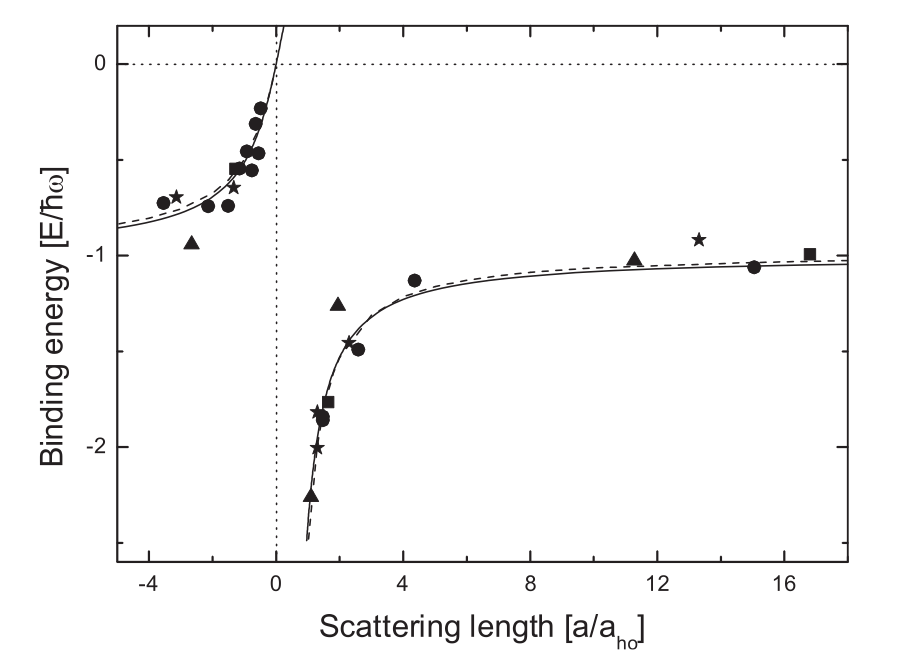
\includegraphics[width=0.5\textwidth]{chap13dmol.png}
    \bicaption{三维光晶格中的Feshbach分子态。散点代表不同晶格深度的实验数据。实线代表理论数据。摘自 \citep{Esslinger3DMol}}{The measured binding energy of molecules in a 3D optical lattice. Scatterd points for defferent depth of latice. The solid line for theory. Reprinted from \citep{Esslinger3DMol}}
    \label{3dmol}
\end{figure}
实验观测到了较深光晶格内调节磁场形成的Feshbach分子态。
%%%%%%%%%%%%%%%%%%%%%%%%%%%%%%%%%%%%%%%%%%%%%%%%%%%%%%%%%%%%%%%%%%%%%%%%%%
\end{comment}

Serwane F及合作者首先发明了一种可以确定性制备不同原子数目的手段\cite{SerwaneDeterministic},这一思路启发了后续精确制备少体体系并探测量子关联的研究\cite{zurn2012fermionization,WenzFermiSeaOnebyOne,Zurn2013Pairing,MurmannSpinChain,MurmannTwoFermionDoubleWell,RontaniTunneling}。研究者利用能级间距较大的微观束缚阱(mircotrap)与两分量${}^6$Li原子热库接触到热平衡,制备$T/T_F\sim0.08$含有600多个原子的费米球。然后在微观束缚阱内施加磁场梯度,使得阱内一端势能降低,然后绝热地改变微观束缚阱的深度,便可使得原子不断漏出,最终制备了只含有几个原子的少体实际物理体系。如图~\ref{deter}~所示。
%%%%%%%%%%%%%%%%%%%%%%%%%%%%%%%%%%%%%%%%%%%%%%%%%%%%%%%%%%%%%%%%%%%%%%%%%%
\begin{figure}[!htbp]
    \centering
    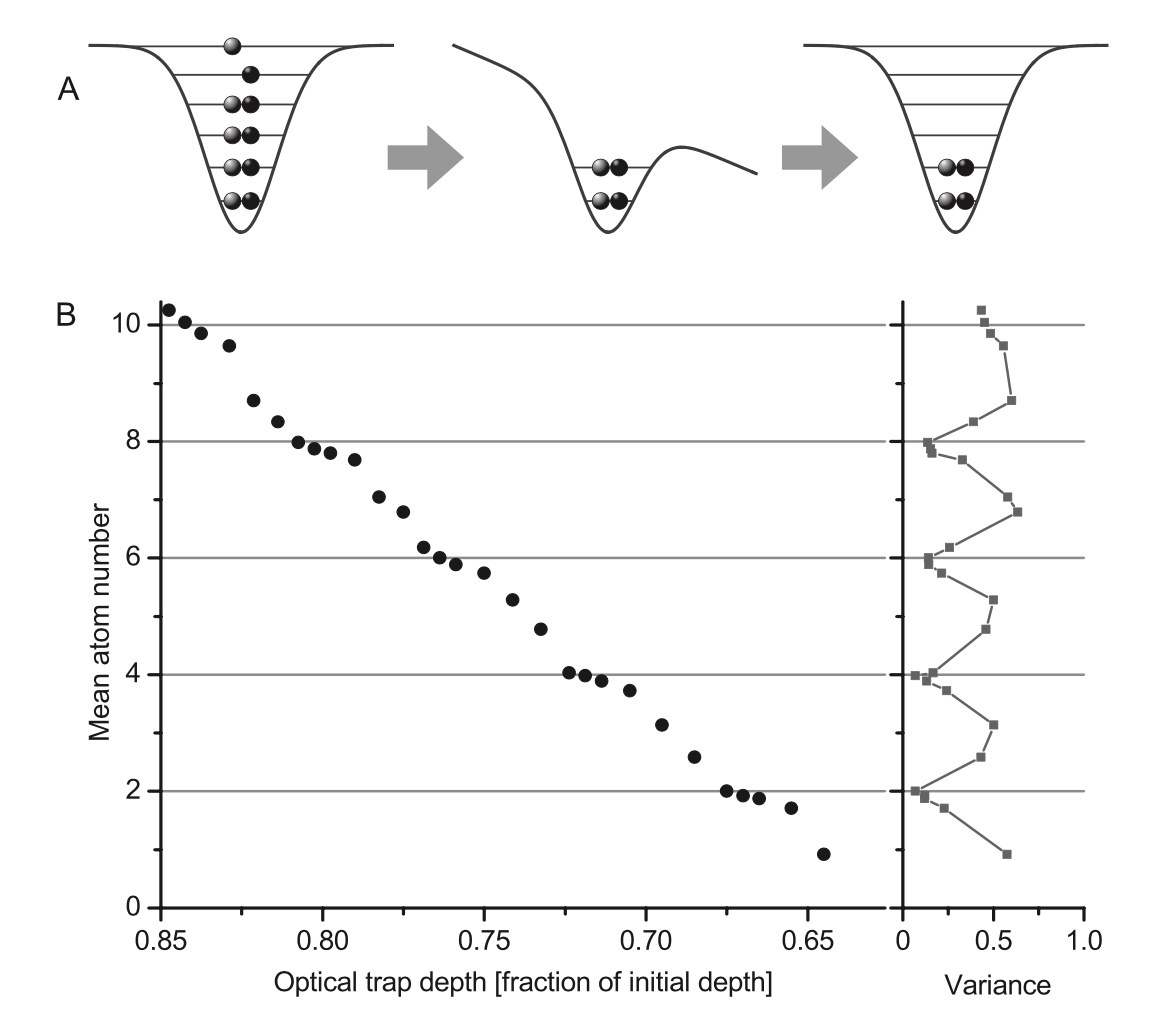
\includegraphics[width=0.5\textwidth]{./intro/chap1deter.png}
    \bicaption{少体体系制备。图A表示降低势阱的示意图,研究者降低一侧势阱深度使原子漏出来制备少体体系。图B为实验测到的少体体系平均粒子数与方差。 摘自 \citep{SerwaneDeterministic} }{Preaparation of few body system. Fig A for illustration of spilling, in which researchers lower potential of one side for atoms spilling. Fig B for measured mean density and variance. Reprinted from\citep{SerwaneDeterministic} }
    \label{deter}
\end{figure}
%%%%%%%%%%%%%%%%%%%%%%%%%%%%%%%%%%%%%%%%%%%%%%%%%%%%%%%%%%%%%%%%%%%%%%%%%%

借助上面精确制备少体体系的方法,研究者研究了不同自旋费米子($\uparrow\downarrow$)之间在强相互作用下发生费米化的过程\cite{zurn2012fermionization}。在准一维束缚阱中制备两体少体体系,调节不同自旋费米子之间的相互作用,通过少体体系隧穿几率反映两体体系的能量。最终得到隧穿几率如图~\ref{ferminization}~
%%%%%%%%%%%%%%%%%%%%%%%%%%%%%%%%%%%%%%%%%%%%%%%%%%%%%%%%%%%%%%%%%%%%%%%%%%
\begin{figure}[!htbp]
    \centering
    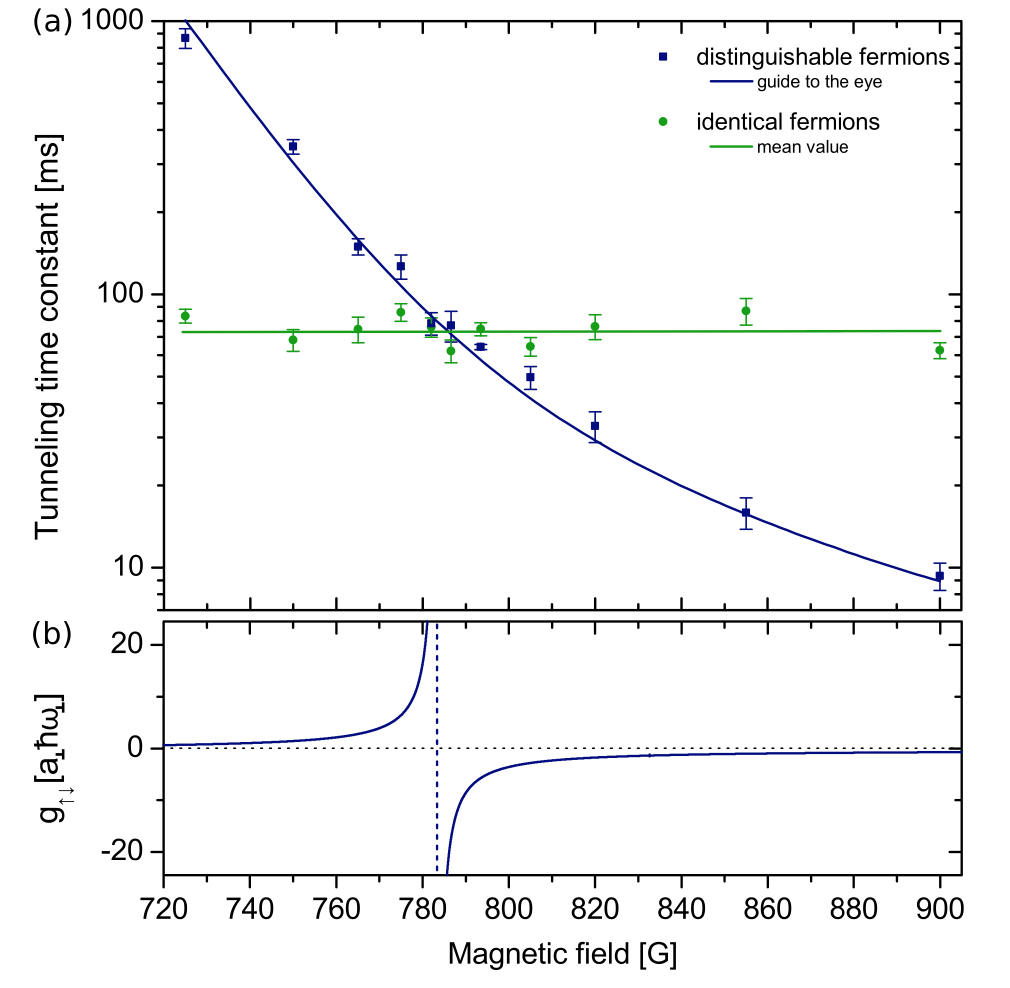
\includegraphics[width=0.5\textwidth]{./intro/chap1ferminization.png}
    \bicaption{不同的有效一维相互作用下两体费米子隧穿几率。谐振子势阱中两体体系的能量决定了隧穿几率。其中在共振点处相互作用费米子$\uparrow\downarrow$能量等于无相互作用全同费米子$\uparrow\uparrow$能量,发生费米化。 摘自 \citep{zurn2012fermionization} }{Tunneling time constant for different 1D effective interaction strengths. Two body energy decides the tunneling time constant. The same tunneling constant of $\uparrow\downarrow$ at resonance point as $\uparrow\uparrow$ reflects the ferminization. Reprinted from\citep{zurn2012fermionization} }
    \label{ferminization}
\end{figure}
%%%%%%%%%%%%%%%%%%%%%%%%%%%%%%%%%%%%%%%%%%%%%%%%%%%%%%%%%%%%%%%%%%%%%%%%%%
所示,同自旋费米子之间无相互作用,调节磁场后两体能级没有变化。但是不同费米子之间相互作用导致散射长度在共振点处发散,对应能量与无相互作用费米子能量相同,体系发生费米化。

进一步地,基于类似的少体制备方法,实验研究者逐步增加粒子数,研究从少体到多体的过渡\cite{WenzFermiSeaOnebyOne}。相关的基本模型为谐振子势阱下N+1的一维极化子物理。相互作用只存在于少数原子与多数原子之间,并且可以通过Feshbach共振调节。从1到5增加多数原子的数目,用射频脉冲测量不同相互作用下极化子的能量,通过与理论计算的1+1与1+$\infty$体系的能量密度进行比较,可以发现在粒子数为5的时候能量密度就很接近多体体系了。如图~\ref{fermisea}~所示。
%%%%%%%%%%%%%%%%%%%%%%%%%%%%%%%%%%%%%%%%%%%%%%%%%%%%%%%%%%%%%%%%%%%%%%%%%%
\begin{figure}[!htbp]
    \centering
    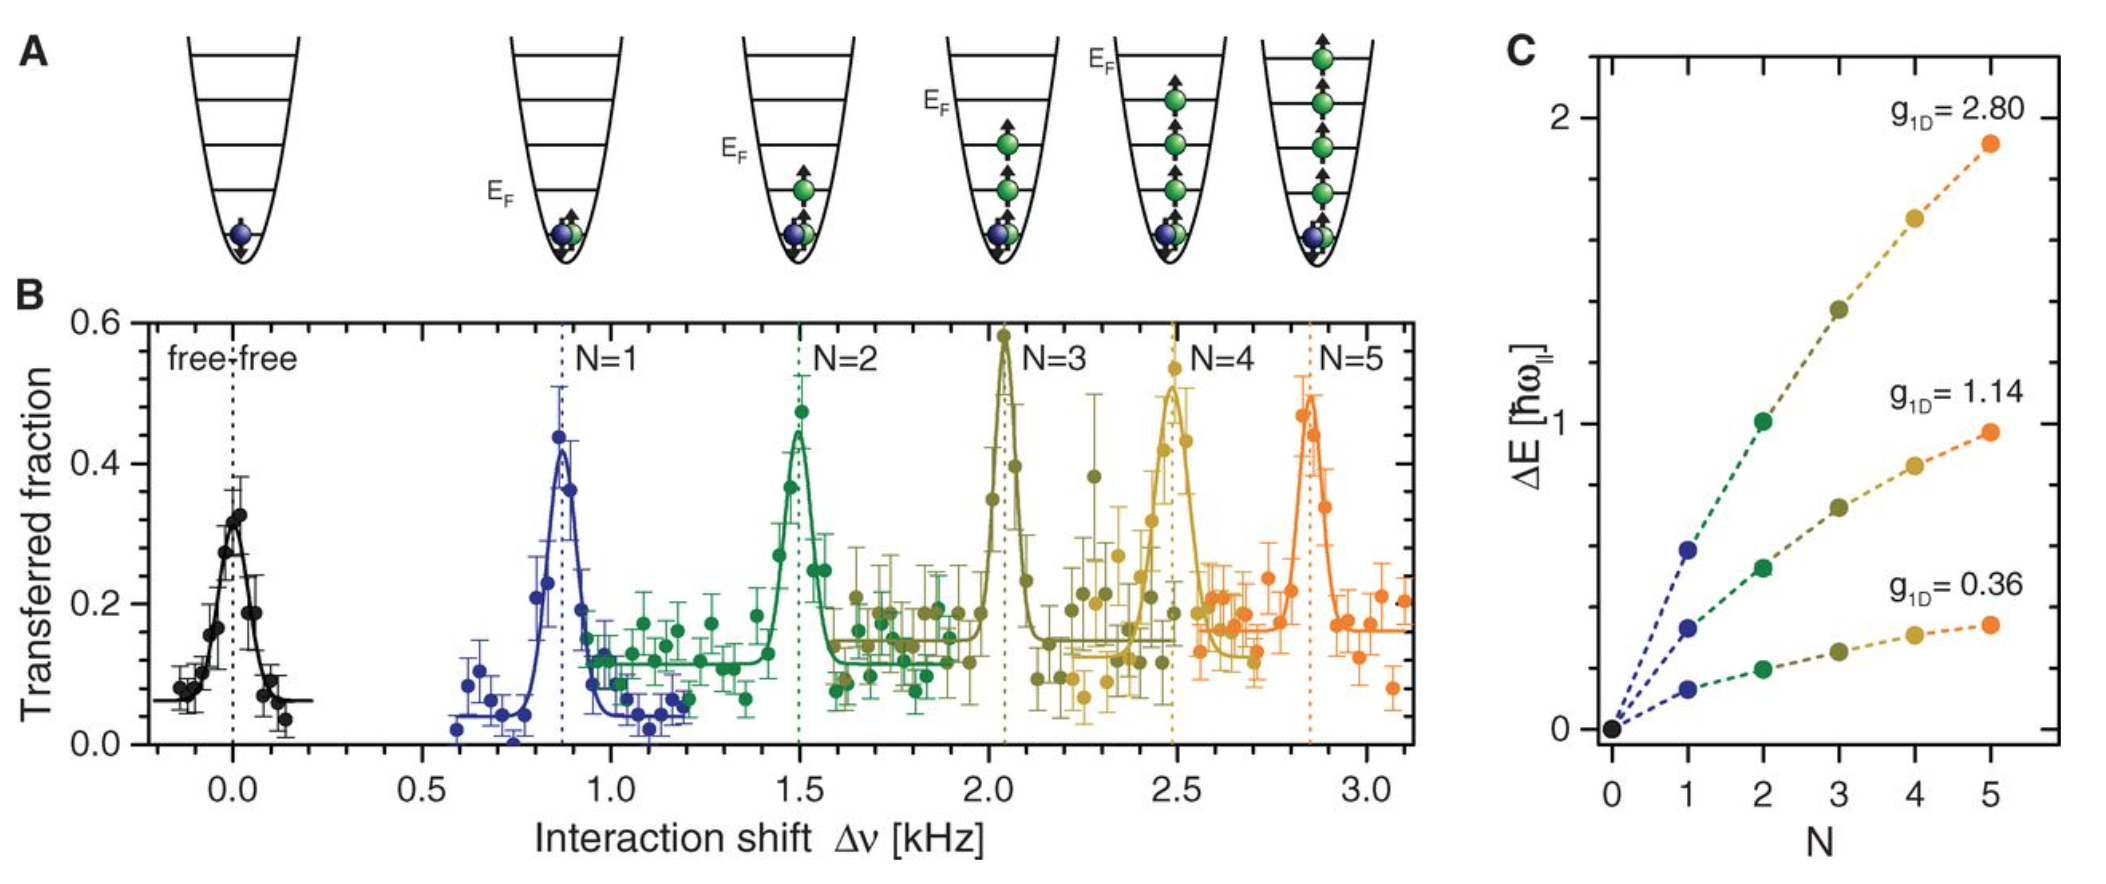
\includegraphics[width=0.8\textwidth]{./intro/chap1fermisea.png}
    \bicaption{ 少体极化子到多体极化子的过渡。图A为谐振子势阱中1+N体系能谱示意图。图B为实验测得的射频脉冲谱。图C为能量密度。摘自 \citep{WenzFermiSeaOnebyOne} }{ Transformation from few body polaron system to many body polaron system. Fig A for energy spectrum of 1+N system. Fig B for measured rf spectrum. Fig C for energy difference. Reprinted from\citep{WenzFermiSeaOnebyOne} }
    \label{fermisea}
\end{figure}
%%%%%%%%%%%%%%%%%%%%%%%%%%%%%%%%%%%%%%%%%%%%%%%%%%%%%%%%%%%%%%%%%%%%%%%%%%

少体物理之所以重要是因为能够在理论方面提供一个可理解的物理图像,在某些特殊极限下甚至存在严格解。这些少体图像构成了我们理解物理的基石。在冷原子领域,有两个经典的两体图像,分别是:自由空间s波散射图像与谐振子势场下s波接触相互作用两体能谱图像。其中前者用来有效地描述相互作用,后者来理解相互作用较强时候系统的能谱与波函数。

1998年, Busch T给出了一个两体体系严格解\cite{busch1998two}:任意维度下两个全同玻色子在谐振子势场下的能谱。虽然是玻色子体系,但是这个严格解同样适用于可分辨费米子。三维情况下,可分辨两体全同费米子位于谐振子外势下,系统的哈密顿量可以写为:
\begin{equation}
\hat{H}=-\frac{1}{2} \nabla_{1}^{2}-\frac{1}{2} \nabla_{2}^{2}+\frac{1}{2} r_{1}^{2}+\frac{1}{2} r_{2}^{2}+4 \pi a_{0} \delta^{(3)}_{reg}\left(\Vector{r}_{1}-\Vector{r}_{2}\right)
\end{equation}
能量量纲为$\hbar\omega$,长度量纲为$\sqrt{\hbar}{m\omega}$,$a_0$代表散射长度。其中$m$为粒子质量,$\omega$为谐振子势场的特征频率,$\delta_{reg}^{(3)}(\Vector{r}) \equiv \delta^{(3)}(\Vector{r})(\partial / \partial r) r$。分离质心运动$\Vector{R}=\sqrt{1 / 2}\left(\Vector{r}_{1}+\Vector{r}_{2}\right)$与相对运动$\Vector{r}=\sqrt{1 / 2}\left(\Vector{r}_{1}-\Vector{r}_{2}\right)$
得到:
\begin{equation}
\begin{aligned}
&\hat{H}_{\mathrm{CM}}=-\frac{1}{2} \nabla_{R}^{2}+\frac{1}{2} \Vector{R}^{2}\\
&\hat{H}_{rel}=-\frac{1}{2} \nabla_{r}^{2}+\frac{1}{2} \Vector{r}^{2}+\sqrt{2} \pi a_{0} \delta^{(3)}(\Vector{r}) \frac{\partial}{\partial r} r\\
\end{aligned}
\end{equation}
质心运动的部分是自由谐振子,剩余相对运动部分满足的薛定谔方程为:
\begin{equation}
\left(\hat{H}_{o s c}+\sqrt{2} \pi a_{0} \delta^{(3)}(\Vector{r}) \frac{\partial}{\partial r} r\right) \Psi(\Vector{r})=E \Psi(\Vector{r})
\end{equation}
相对运动部分的$l\neq0$空间不受相互作用影响,仍为自由谐振子,只考虑$l=0$子空间。波函数展开在谐振子基矢下:
相应的本征波函数为:
\begin{equation}
\Psi(\Vector{r})=\sum_{n=0}^{\infty} c_{n} \varphi_{n}(\Vector{r})
\end{equation}
带入到薛定谔方程里得到:
\begin{equation}
c_{n}\left(E_{n}-E\right)+\sqrt{2} \pi a_{0} \varphi_{n}^{*}(0)\left[\frac{\partial}{\partial r}\left(r \sum_{m=0}^{\infty} c_{m} \varphi_{m}(\Vector{r})\right)\right]_{r \rightarrow 0}=0
\end{equation}
求得$c_n$满足:
\begin{equation}
c_{n}=A \frac{\varphi_{n}^{*}(0)}{E_{n}-E}
\end{equation}
将系数带回到薛定谔方程得到本征能量满足:
\begin{equation}
\sqrt{2} \frac{\Gamma(-E / 2+3 / 4)}{\Gamma(-E / 2+1 / 4)}=\frac{1}{a_{0}}
\end{equation}
对应的本征波函数解析形式为:
\begin{equation}
\Psi(\Vector{r})=\frac{1}{2} \pi^{-3} / 2 A e^{-r^{2} / 2} \Gamma(-v) U\left(-v, \frac{3}{2}, r^{2}\right)
\end{equation}
其能谱随着散射长度变化如图~\ref{chap1busch}~所示:
%%%%%%%%%%%%%%%%%%%%%%%%%%%%%%%%%%%%%%%%%%%%%%%%%%%%%%%%%%%%%%%%%%%%%%%%%%
\begin{figure}[!htbp]
    \centering
    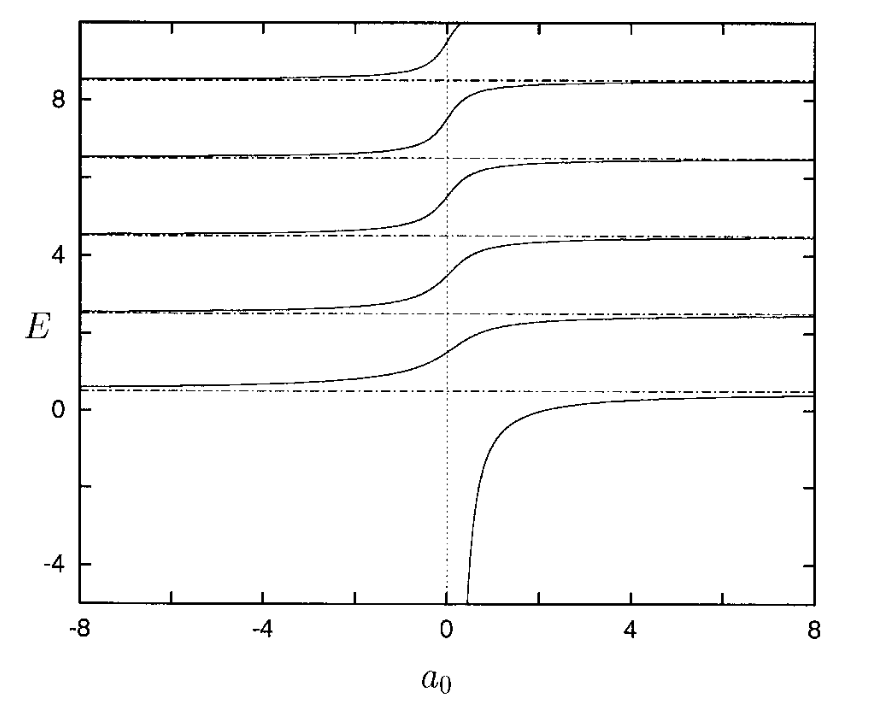
\includegraphics[width=0.6\textwidth]{./intro/chap1busch.png}
    \bicaption{三维下$l=0$空间的两体能谱。摘自\citep{busch1998two} }{Two body spectrum in 3D. Reprinted from \citep{busch1998two} }
    \label{chap1busch}
\end{figure}
%%%%%%%%%%%%%%%%%%%%%%%%%%%%%%%%%%%%%%%%%%%%%%%%%%%%%%%%%%%%%%%%%%%%%%%%%%
当$a_0\to \infty$时候,基态能量渐近行为是$E_g\propto - 1/a_0^2$,称为吸引低能支(attractive lower branch);其余的随着$a_0\to\infty$本征能量饱和在奇数谐振子能量的态称为排斥高能支(repulsive upper branch)。这个少体体系的严格解在后续的实验与理论发展中起了很重要的作用。

类似地,一维以及二维的结果也可用上述求解过程给出。其中一维的能量方程与三维相同,不同在于仅满足偶宇称的解受到相互作用影响。二维下能量方程则有很大不同:
\begin{equation}
\psi(-E / 2+1 / 2)=\log \left(\frac{1}{2 a_{0}^{2}}\right)
\end{equation}

后续对这个体系的严格解有了一些扩展,主要是各向异性的谐振子外势求解,以及动力学研究,更多详细内容请参见\cite{blume2012few}。

如果再增加一个粒子,这个三体体系则没有解析解,只能通过数值手段去求解。我们以$\uparrow\downarrow\uparrow$的费米子三体体系为例,仅在不同自旋费米子之间有s波散射相互作用\cite{OlshaniiRigorous2001,Petrov2003unitary3b,Fleix2006prlunitary3b,Felix2006praunitary3b,LmDuan2007levelcrossing,Stetcu2007,Blume2008,Blume2010,Xiaji2009prl,Xiaji20103b,Rittenhouse2010green}。我们用Bethe-Peierls条件代替相互作用:
\begin{equation}
\psi\left(\Vector{r}_{1}, \Vector{r}_{2}, \Vector{r}_{3}\right)=\left(\frac{1}{r_{i j}}-\frac{1}{a}\right) A\left(\Vector{R}_{i j}, \Vector{r}_{k}\right)+O\left(r_{i j}\right)
\end{equation}
其中$r_{i j} \equiv\left|\Vector{r}_{i}-\Vector{r}_{j}\right| \rightarrow 0$,$\Vector{R}_{ij}$为两原子的质心位置。

\begin{comment}
三维情况下这种体系的求解\cite{Fleix2006prlunitary3b}借助于超球(Hypersphere)框架,先引入Jacobi坐标:
\begin{equation}
\begin{split}
\Vector{r}&=\Vector{r}_{2}-\Vector{r}_{1}\\
\boldsymbol{\rho}&=\left(2 \Vector{r}_{3}-\Vector{r}_{1}-\Vector{r}_{2}\right) / \sqrt{3}\\
\Vector{C}&=\left(\Vector{r}_{1}+\Vector{r}_{2}+\Vector{r}_{3}\right) / 3\\
\end{split}
\end{equation}
然后定义超半径(hyperradius)与超角度(hyperangle):
\begin{equation}
\begin{split}
R&=\sqrt{\left(r^{2}+\rho^{2}\right) / 2}\\
\alpha&=\arctan (r / \rho)\\
\end{split}
\end{equation}
这时候谐振子外势只出现在$R$的薛定谔方程中。考虑波函数形式:
\begin{equation}
\psi\left(\Vector{r}_{1}, \Vector{r}_{2}, \Vector{r}_{3}\right)=\psi_{\mathrm{c} . \mathrm{m} .}(\Vector{C}) F(R)(1+\hat{Q}) \frac{1}{r \rho} \varphi(\alpha) Y_{l}^{m}(\boldsymbol{\rho} / \rho)
\end{equation}
其中$Y_l^m$为角动量为$l$的球谐函数。$l$为三体内部相对角动量。$\hat{Q}=-\hat{P}_{13}$将上式带入薛定谔方程得到$\alpha$满足:
\begin{equation}
\begin{gathered}
-\varphi^{\prime \prime}(\alpha)+\frac{l(l+1)}{\cos ^{2} \alpha} \varphi(\alpha)=s^{2} \varphi(\alpha) \\
\varphi(\pi / 2)=0 \\
\varphi^{\prime}(0)+\eta(-1)^{l} \frac{4}{\sqrt{3}} \varphi(\pi / 3)=0
\end{gathered}
\end{equation}
其中$\eta=-1$。对任意$l$,可以解得一系列$s_{l,n},n=0,1,2,3...$均为实数。如图~\ref{Sv}~
\begin{figure}[!htbp]
    \centering
    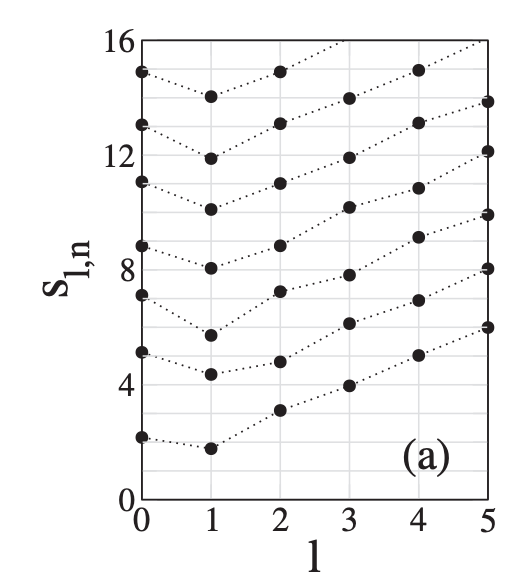
\includegraphics[width=0.5\textwidth]{chap13fSv.png}
    \bicaption{幺正极限下$\uparrow\downarrow\uparrow$三体体系$s_{l,n}$数值结果。摘自\citep{Fleix2006prlunitary3b} }{Numerical $s_{l,n}$ of $\uparrow\downarrow\uparrow$ three fermion system under unitary limit. Reprinted from \citep{Fleix2006prlunitary3b}}
    \label{Sv}
\end{figure}
将解到的$s_{l,n}$带入:
\begin{equation}
\left[-\frac{\hbar^{2}}{2 m}\left(\frac{d^{2}}{d R^{2}}+\frac{1}{R} \frac{d}{d R}\right)+U(R)\right] F(R)=\left(E-E_{\mathrm{c} . \mathrm{m} .}\right) F(R)
\end{equation}
其中$U(R)=\hbar^{2} s^{2} /\left(2 m R^{2}\right)+m \omega^{2} R^{2} / 2$。即可求得三体本征解。

基于上述框架,当s波相互作用处于幺正极限$a\to+\infty$时候,我们可以得到解析解,本征波函数为:
\begin{equation}
 F(R)=R^{s} e^{-R^{2} / 2 a_{\mathrm{ho}}^{2}} L_{q}^{(s)}\left(R^{2} / a_{\mathrm{ho}}^{2}\right)
\end{equation}
其中$a_{ho}=\sqrt{\hbar/m\omega}$,$s$为其中一个$s_{l,n}$,$L^{(\cdot)}_q$为q阶广义拉盖尔多项式,$q$为任意非负整数。能谱为:
\begin{equation}
E=E_{\mathrm{c} . \mathrm{m} .}+\left(s_{l, n}+1+2 q\right) \hbar \omega
\end{equation}

对于非幺正极限的相互作用情况,只能完全借助数值方法。Duan\cite{LmDuan2007levelcrossing}用格林函数的方法数值求解了整个相互作用区间。与上述框架稍有不同,哈密顿量为:
\begin{equation}
\begin{aligned}
&{\left[-\frac{\hbar^{2}}{m_{0}}\left(\nabla_{\Vector{x}}^{2}+\nabla_{\Vector{y}}^{2}\right)+\frac{1}{4} m_{0} \omega^{2}\left(\Vector{x}^{2}+\Vector{y}^{2}\right)-E\right] \Psi(\Vector{x}, \Vector{y})} \\
&\quad=-\sum V\left(\Vector{r}_{\pm}\right) \Psi(\Vector{x}, \Vector{y})
\end{aligned}
\end{equation}
其中$\Vector{y}$为两个$\uparrow$费米子间相对位置。$\frac{\sqrt{\Vector{x}}}{2}$为$\downarrow$费米子相对两$\uparrow$费米子质心的相对位置。波函数在氢原子本征基矢下下展开,求解格林函数并利用边界条件,其中$\Vector{r}_{\pm}=\sqrt{3} \Vector{x} / 2 \pm \Vector{y} / 2$。
\begin{equation}
\begin{aligned}
&\Psi(\Vector{x}, \Vector{y})= \int d \Vector{x}^{\prime} d \Vector{y}^{\prime} G_{E}^{(2)}\left(\Vector{x}, \Vector{y} ; \Vector{x}^{\prime}, \Vector{y}^{\prime}\right)\times \sum_{\pm} \frac{\mp \hbar^{2} f\left(\Vector{r}^{\prime}{ }_{\perp, \pm}\right)}{m_{0}} \delta\left(\Vector{r}^{\prime}{ }_{\pm}\right)\\
&G_{E}^{(2)}\left(\Vector{x}, \Vector{y} ; \Vector{x}^{\prime}, \Vector{y}^{\prime}\right)=\sum_{\lambda_{1} \lambda_{2}} \frac{\psi_{\lambda_{1}}(\Vector{x}) \psi_{\lambda_{2}}(\Vector{y}) \psi_{\lambda_{1}}^{*}\left(\Vector{x}^{\prime}\right) \psi_{\lambda_{2}}^{*}\left(\Vector{y}^{\prime}\right)}{E_{\lambda_{1}}+E_{\lambda_{2}}-E}\\
\end{aligned}
\end{equation}
其中$\psi_\lambda(\Vector{r}) = R_{nl}(r)Y_l^m(\theta,\phi)$,$\lambda = (n,l,m),n=0,1,2...,l=0,1,2...$,$\Vector{r}_{\perp, \pm}=\Vector{x} / 2 \mp \sqrt{3} \Vector{y} / 2$边界条件为:
\begin{equation}
\Psi(\Vector{x}, \Vector{y}) \simeq \mp \frac{f\left(\Vector{r}_{\perp, \pm}\right)}{4 \pi \Vector{r}_{\pm}}\left(1-\frac{\Vector{r}_{\pm}}{a}\right) \text { for } \Vector{r}_{\pm} \rightarrow 0
\end{equation}
进一步将$f\left(\Vector{r}_{\perp}\right)$展开:
\begin{equation}
f\left(\Vector{r}_{\perp}\right)=\Sigma_{\lambda} f_{\lambda} \psi_{\lambda}\left(\Vector{r}_{\perp}\right)
\end{equation}
得到$f_\lambda$满足的矩阵方程:
\begin{equation}
\sum_{\lambda^{\prime}} A_{\lambda^{\prime}} f_{\lambda^{\prime}}=\left[\frac{d}{a}-2 \frac{\Gamma\left(\frac{3 / 2+E_{\lambda} / \hbar \omega-E / \hbar \omega}{2}\right)}{\Gamma\left(\frac{1 / 2+E_{\lambda} / \hbar \omega-E / \hbar \omega}{2}\right)}\right] f_{\lambda},
\end{equation}
其中:
\begin{equation}
A_{\lambda \lambda^{\prime}}=\int \frac{d \Vector{r}_{\perp}}{4 \pi d^{3} \hbar \omega} G_{E-E_{\lambda^{\prime}}}\left(\frac{\sqrt{3} \Vector{r}_{\perp}}{2}, 0\right) \psi_{\lambda}^{*}\left(\Vector{r}_{\perp}\right) \psi_{\lambda^{\prime}}\left(\frac{-\Vector{r}_{\perp}}{2}\right)
\end{equation}
最终得到能谱如图~\ref{duancrossing}~所示,通过跟两体能量的比较作者进一步发现了能级交叉。
\begin{figure}[!htbp]
    \centering
    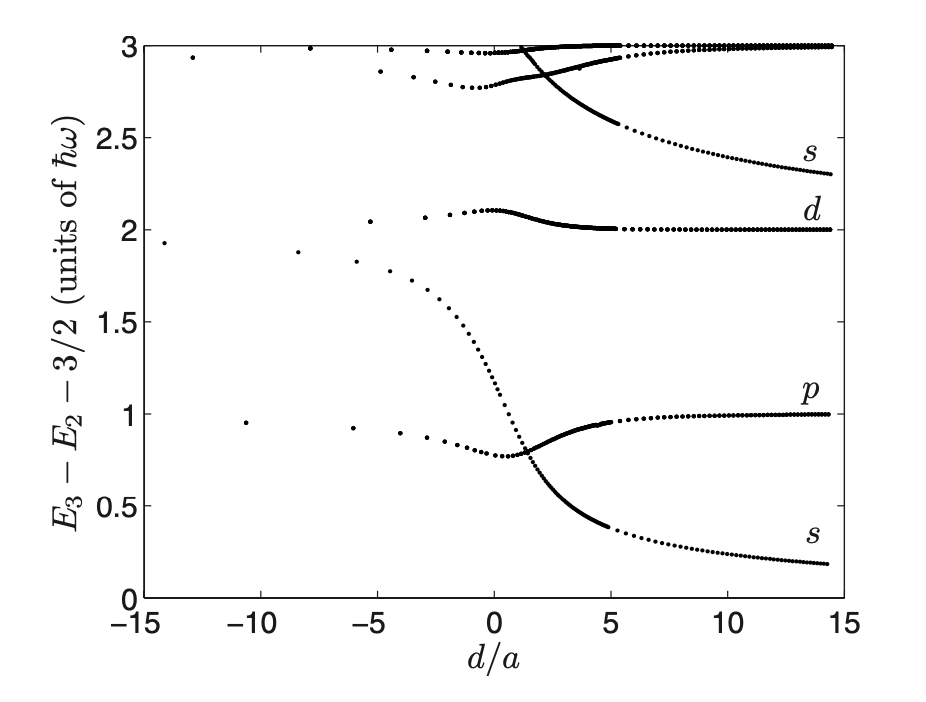
\includegraphics[width=0.7\textwidth]{chap1duan.png}
    \bicaption{三维下三费米子体系($\uparrow\downarrow\uparrow$)能谱。摘自\citep{LmDuan2007levelcrossing}}{Spectrum
     of three fermions system($\uparrow\downarrow\uparrow$)in 3D. Reprinted from \citep{LmDuan2007levelcrossing}}
    \label{duancrossing}
\end{figure}
\end{comment}

三体体系的求解用到两体本征波函数作为基矢\cite{Xiaji2009prl},三体波函数为:
\begin{equation}
\begin{split}
\psi_{3 b}^{\mathrm{rel}}(\Vector{r}, \rho)&=\left(1-\mathcal{P}_{13}\right) \chi(\Vector{r}, \rho)\\
\chi(\Vector{r}, \rho)&=\sum a_{n} \psi_{2 b}^{\mathrm{rel}}\left(r ; v_{l, n}\right) R_{n l}(\rho) Y_{l}^{m}(\hat{\rho})\\
\end{split}
\end{equation}
其中$\psi_{2 b}^{\mathrm{rel}}$代表费米子1,2相对运动的波函数,对应能量为$E_{2b}=(2v_{l,n}+3/2)\hbar\omega$,而$R_{nl}(\rho Y^m_l(\hat{\rho}))$,其中$l,m$是系统的好量子数,代表了相对角动量与其沿z方向的分量。其物理图像非常清晰,将其中一个$\uparrow$费米子与$\downarrow$费米子结合在一起成为二聚体,第三个费米子相对于这个二聚体的运动由$a_n$所描述。最终求解方程:
\begin{equation}
\begin{split}
&\frac{2 \Gamma\left(-v_{l, n}\right)}{\Gamma\left(-v_{l, n}-1 / 2\right)} a_{n}+\frac{(-1)^{l}}{\sqrt{\pi}} \sum_{n^{\prime}} C_{n n^{\prime}} a_{n^{\prime}}=\left(\frac{d}{a}\right) a_{n}\\
&C_{n n^{\prime}} \equiv \int_{0}^{\infty} \rho^{2} d \rho R_{n l}(\rho) R_{n^{\prime} l}\left(\frac{\rho}{2}\right) \psi_{2 b}^{\mathrm{rel}}\left(\frac{\sqrt{3} \rho}{2} ; v_{l, n^{\prime}}\right)\\
\end{split}
\end{equation}
其能谱如图~\ref{xiaji3d}~所示。
%%%%%%%%%%%%%%%%%%%%%%%%%%%%%%%%%%%%%%%%%%%%%%%%%%%%%%%%%%%%%%%%%%%%%%%%%%
\begin{figure}[!htbp]
    \centering
    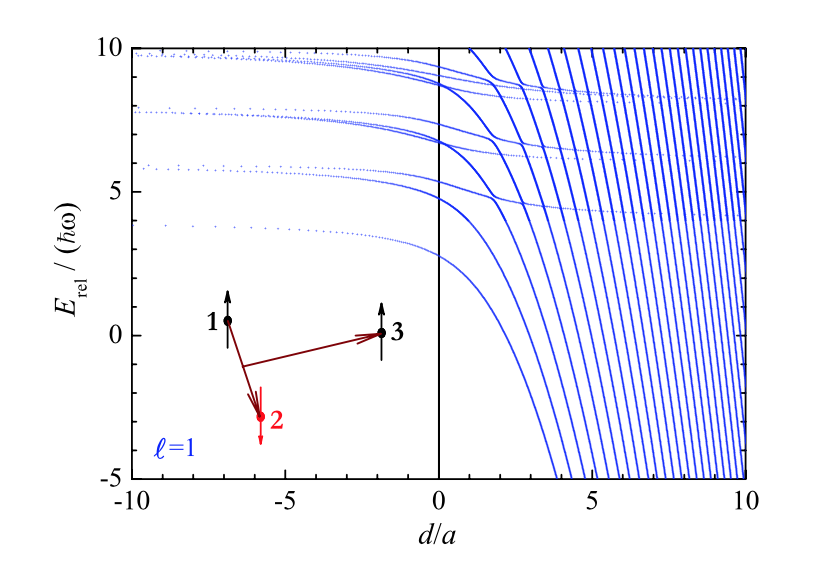
\includegraphics[width=0.6\textwidth]{./intro/chap1xiaji.png}
    \bicaption{三维下三费米子体系($\uparrow \downarrow \uparrow$)的能谱。摘自\citep{Xiaji2009prl}}{Spectrum of three fermions system($\uparrow\downarrow\uparrow$) in 3D. Reprinted from \citep{Xiaji2009prl}}
    \label{xiaji3d}
\end{figure}
%%%%%%%%%%%%%%%%%%%%%%%%%%%%%%%%%%%%%%%%%%%%%%%%%%%%%%%%%%%%%%%%%%%%%%%%%%
后续研究者\cite{Xiaji20103b}还研究了二维体系下三体精确解,采用类似的基矢展开,
\begin{equation}
\begin{split}
\psi_{3 f}^{r e l}&=\left(1-\mathcal{P}_{13}\right) \chi(\Vector{r}, \vec{\rho})\\
\chi(\Vector{r}, \vec{\rho})&=\sum_{n} a_{n}^{f} \psi_{2 p}^{r e l}\left(\Vector{r} ; \nu_{m, n}\right) R_{n m}(\rho) \frac{e^{i m \varphi}}{\sqrt{2 \pi}}\\
\end{split}
\end{equation}
得到整个相互作用区间的的能谱。同时研究者研究了从三维到二维一维的渡越\cite{blume2012},通过各向异性的谐振子束缚体系的求解来研究维度的渡越。而在严格一维体系里面,三费米子的严格求解则由\cite{Rittenhouse2010green,d2014three,loft2015variational,andersen2016interpolatory,bellotti2017comparing}给出。
采用的波函数为:
\begin{equation}
\begin{split}
\psi_{3 F}(x, y)&=\left(1-\boldsymbol{P}_{13}\right) \Omega(x, y)\\
\Omega(x, y)&=\sum_{n=0}^{\infty} a_{n} \psi_{n}^{2b}(x) R_{n}(y)\\
\psi_{n}^{2b}(x)&=\Gamma\left(-v_{n}\right) \mathrm{e}^{-\frac{x^{2}}{2}} U\left(-v_{n}, \frac{1}{2}, x^{2}\right)\\
\end{split}
\end{equation}
其中$\psi_{n}^{2b}(x)$为两体相互作用在谐振势中的解,$R_{n}(y)$为谐振子的本征解。类似地,带入到Bethe–Peierls边界条件中得到耦合方程:
\begin{equation}
\begin{aligned}
&2 g \sum_{n} a_{n}\left[\sqrt{\pi} \frac{\Gamma\left(-v_{n}\right)}{\Gamma\left(-v_{n}+1 / 2\right)} R_{n}(y)-\psi_{n}\left(\frac{\sqrt{3}}{2} y\right) R_{n}\left(-\frac{y}{2}\right)\right] \\
&=-4 \sqrt{\pi} \sum_{n} a_{n} R_{n}(y)
\end{aligned}
\end{equation}
其能谱结构与三维下三体能谱类似。

\begin{comment}
相应地能谱如图~\ref{1d3b}~所示。
%%%%%%%%%%%%%%%%%%%%%%%%%%%%%%%%%%%%%%%%%%%%%%%%%%%%%%%%%%%%%%%%%%%%%%%%%%
\begin{figure}[!htbp]
    \centering
    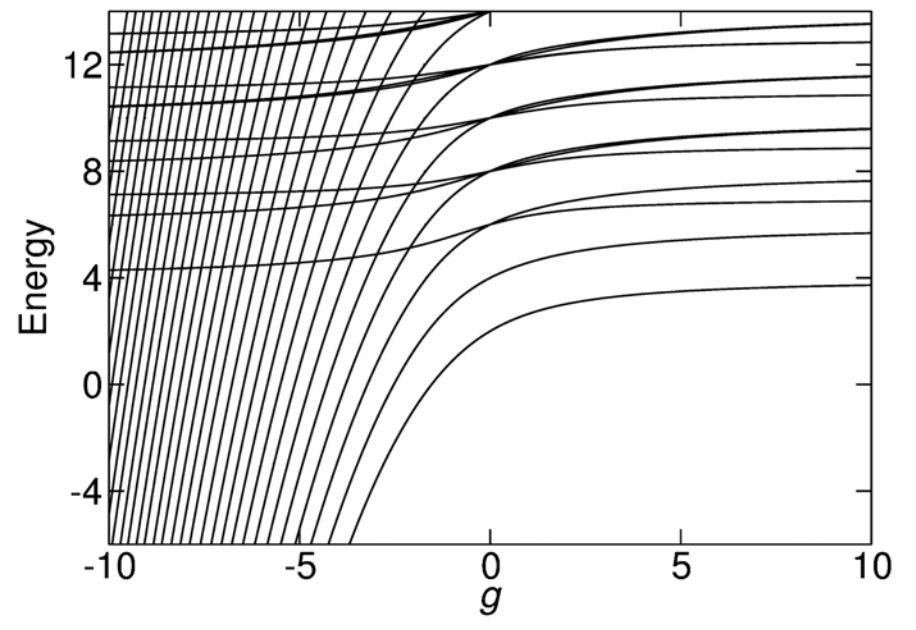
\includegraphics[width=0.7\textwidth]{chap11d3b.png}
    \bicaption{一维下三费米子体系$\uparrow \downarrow \uparrow$的能谱。摘自\citep{d2014three} }{Spectrum of three fermion system($\uparrow\downarrow\uparrow$ in 1D. Reprinted from \citep{d2014three}}
    \label{1d3b}
\end{figure}
%%%%%%%%%%%%%%%%%%%%%%%%%%%%%%%%%%%%%%%%%%%%%%%%%%%%%%%%%%%%%%%%%%%%%%%%%%
\end{comment}

继续增加粒子的数目到四体甚至五体,有一些数值结果\cite{Blume2010,blume2012few},不过如何有效地求解这类体系依然是一个开放问题。多粒子体系中唯一的例外就是在严格一维时候,可以利用贝特假设严格求解,通常情况下贝特假设结果的物理意义不容易提取,但是在某些极限下却有清楚的物理图像,这其中一个典型例子就是Tonks极限及其附近的自旋链模型\cite{Guan2009exact,ma2009mathematical,Lewenstein2013spinchain,volosniev2014strongly,Busch013spinchain,CuiHo2014,Santos2014spinchain,Puhan2015spinchain,Yang2016effective}。
这一模型最早在冷原子少体物理中得以实现,制备$(N_\uparrow,N_\downarrow)=(2,1,(3,1),(2,2)$少体体系,绝热地调节不同自旋之间相互作用从自由极限到Tonks极限,越过共振点进入super Tonks极限,制备了反铁磁自旋链与铁磁自旋链,其中蕴含的少体关联也直接由实验成功探测\citep{MurmannSpinChain}。

\begin{comment}
\begin{figure}[!htbp]
    \centering
    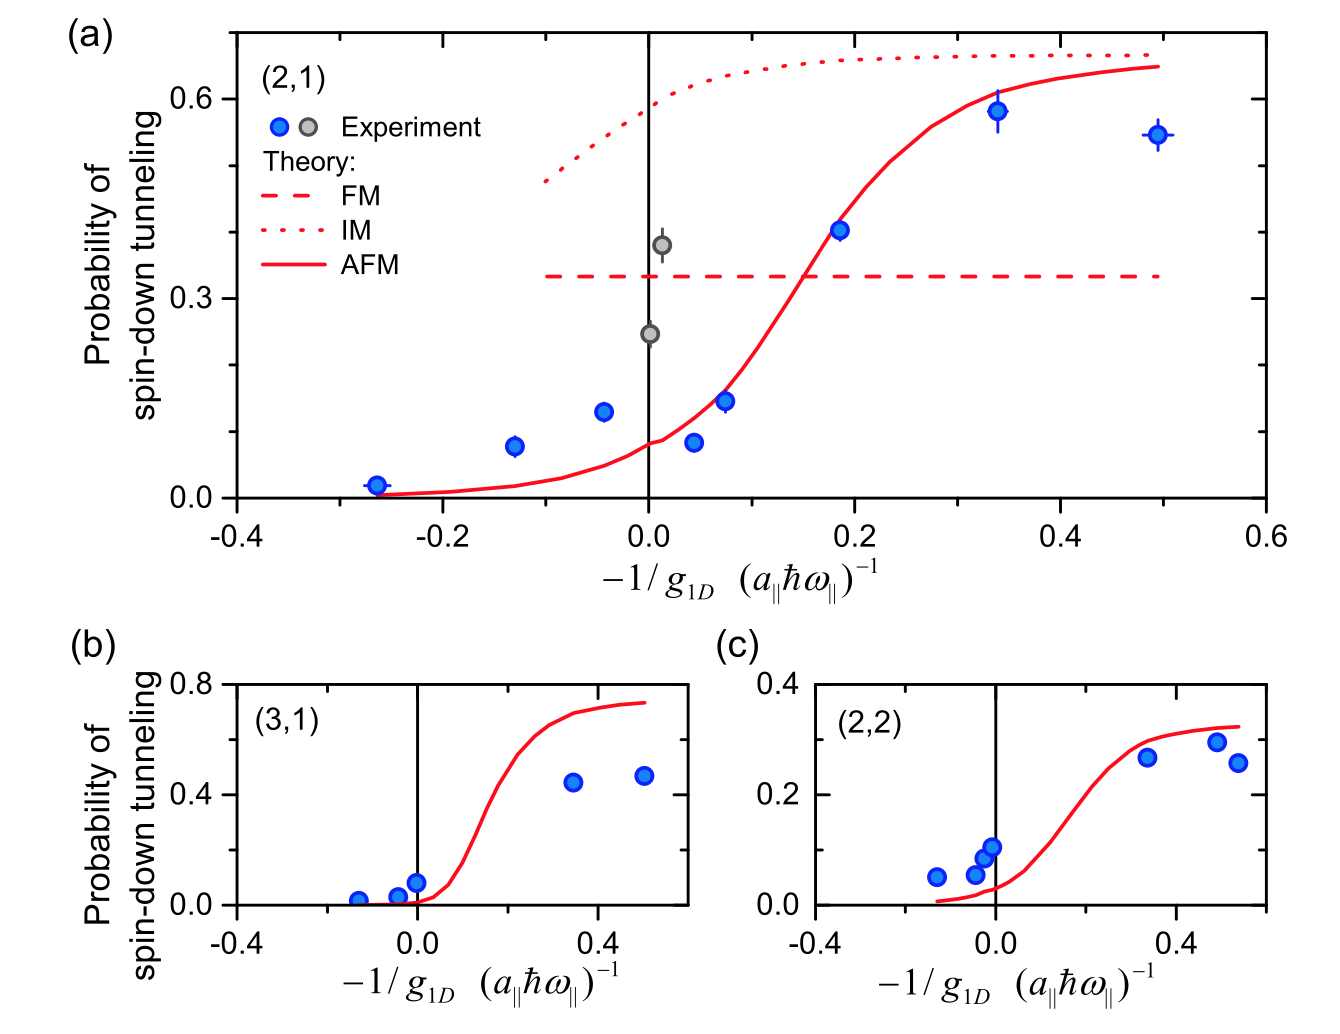
\includegraphics[width=0.7\textwidth]{chap1spinchain.png}
    \bicaption{ 不同少体体系$\downarrow$原子隧穿几率随一维有效相互作用的变化,a为(2,1),b为(3,1),c为(2,2)。散点为实验测得数据。线条代表不同的自旋链模型计算得到的隧穿几率。摘自 \citep{MurmannSpinChain} }{Tunneling rate of $\downarrow$ atom in different few body systems upon 1D effective coupling constant. a for (2,1), b for (3,1) and cc for (2,2). Reprinted from\citep{MurmannSpinChain} }
    \label{chap1spinchainexp}
\end{figure}
%%%%%%%%%%%%%%%%%%%%%%%%%%%%%%%%%%%%%%%%%%%%%%%%%%%%%%%%%%%%%%%%%%%%%%%%%%
实验上通过让边缘处的粒子漏出,来测量自旋分布。漏出的几率由初态能量与末态能量决定。通过与理论自旋链模型的漏出几率对比,可以确认制备到反铁磁自旋链。如图~\ref{chap1spinchainexp}~所示。
\end{comment}

理论方面,对于无限大相互作用的自旋1/2费米子体系的研究则受到Girardeau处理玻色子的启发,研究者求解了带有自旋费米子体系的严格解\cite{Guan2009exact},其中基态简并是一重要特征。定义N个费米子在一维顺序自旋排布$\xi_{1}, \xi_{2}, \ldots, \xi_{N}$态为:
\begin{equation}
\left|\left\{\xi_{1}, \xi_{2}, \ldots, \xi_{N}\right\}\right\rangle \equiv|\vec{\xi}\rangle
\end{equation}
其坐标表示为:
\begin{equation}
\begin{aligned}
&\langle x_{1}, \ldots, x_{N} ; \mu_{1}, \ldots, \mu_{N} \mid \vec{\xi}\rangle \\
&\quad=\sum_{P} \theta\left(x_{P_{1}}, x_{P 2}, \ldots, x_{P_{N}}\right) \prod_{i} \delta_{\xi_{i}, \mu_{P_{i}}}
\end{aligned}
\end{equation}
其中$P$为$(1,2..,N)$的一个置换。并且:
\begin{equation}
\begin{aligned}
\theta\left(x_{P_{1}}, x_{P 2}, \ldots, x_{P_{N}}\right) &=1 & & \text { 如果 } x_{P_{1}}<x_{P 2}<\cdots<x_{P_{N}} \\
&=0 & & \text { 其它 }
\end{aligned}
\end{equation}
由于体系相互作用仅存在于不同自旋费米子之间,因此总的自旋$\Vector{S}_{tot},S_{tot,z}$守恒。N个费米子在共振点处发生费米化,相互作用转变为边界条件:
\begin{equation}
\left.\Psi\left(x_{1}, \sigma_{1} ; \ldots ; x_{N}, \sigma_{N}\right)\right|_{x_{i}=x_{j}, \sigma_{i}=-\sigma_{j}}=0
\end{equation}
如果其中$M$个$\uparrow$,$N-M$个$\downarrow$,本征波函数具有$C_N^M$重简并:
\begin{equation}
\begin{split}
&\Psi_{F}^{\xi}=\phi_{F}\left(x_{1}, x_{2}, \ldots, x_{N}\right)\langle x_{1}, \ldots, x_{N} ; \mu_{1}, \ldots, \mu_{N} \mid \vec{\xi}\rangle\\
&\phi_{F}\left(x_{1}, x_{2}, \ldots, x_{N}\right) =\frac{1}{\sqrt{N !}} D\left(x_{1}, x_{2}, \ldots, x_{N}\right) \\
&\quad\quad =\prod_{i<j}\left(x_{i}-x_{j}\right) F\left(x_{1}, x_{2}, \ldots, x_{N}\right)\\
\end{split}
\end{equation}
其中$\phi_F$由N个不同谐振子能级构成。一旦相互作用不在共振处,这些简并的能级就会打开简并,其打开简并的方式恰好可以被自旋链模型所描述。
\begin{equation}
\hat{H}_{\mathrm{eff}}=\sum_{l} \frac{J_{l}}{g}\left(\Vector{s}_{l} \cdot \Vector{s}_{l+1}-\frac{1}{4}\right)
\end{equation}
其中自旋之间的耦合常数满足:
\begin{equation}
J_{l}=\left.2 N !\left(\frac{1}{m}\right)^{2} \int d \Vector{x}\left|\frac{\partial \phi_{F}}{\partial x_{i j}}\right|_{x_{i j}=0}\right|^{2} \theta\left(\cdots<x_{i}=x_{j}<\cdots\right)
\end{equation}
具体的计算参见\cite{Guan2009exact,Santos2014spinchain,Yang2016effective}
%%%%%%%%%%%%%%%%%%%%%%%%%%%%%%%%%%%%%%%%%%%%%%%%%%%%%%%%%%%%%%%%%%%%%%%%%%
\begin{figure}[!htbp]
    \centering
    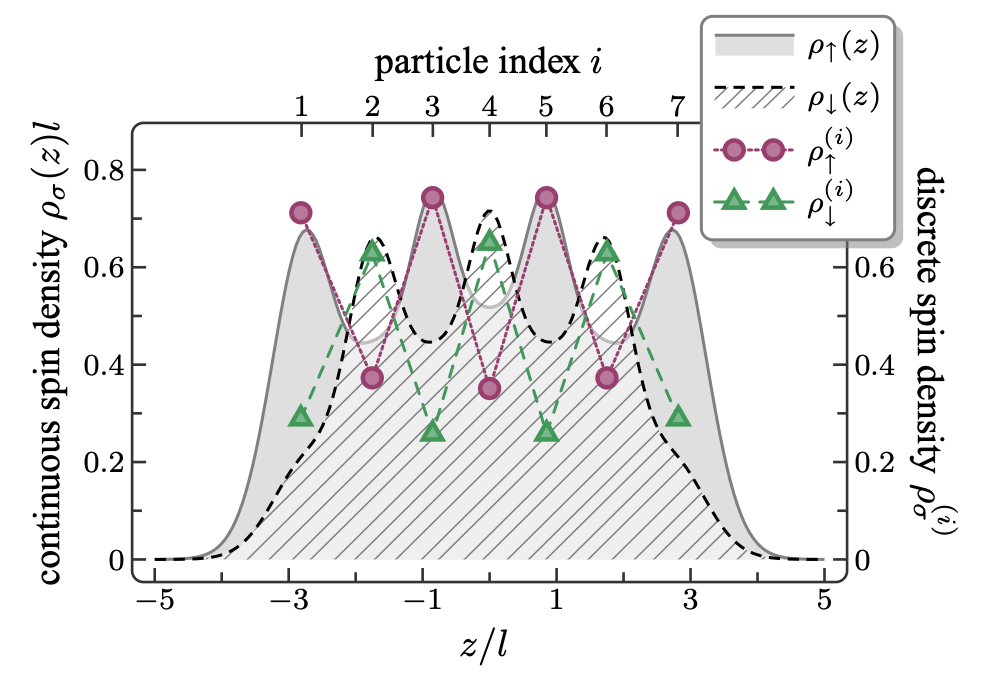
\includegraphics[width=0.6\textwidth]{./intro/chap1spinchainth.png}
    \bicaption{少体自旋1/2费米子体系无限大排斥附近的自旋链有效模型。摘自\citep{Santos2014spinchain} }{Spin-chain representation of an infinitely repulsive system of a few fermions. Reprinted from \citep{Santos2014spinchain}}
    \label{spinchainth}
\end{figure}
%%%%%%%%%%%%%%%%%%%%%%%%%%%%%%%%%%%%%%%%%%%%%%%%%%%%%%%%%%%%%%%%%%%%%%%%%%
\begin{comment}
基于上面介绍的量子少体研究进展,将有几个可扩展的方向,比如改变相互作用,偶极、库伦、以及自旋交换相互作用,这其中自旋交换相互作用将是下一章节要重点介绍的。
\end{comment}











\section{自旋交换相互作用}\label{1sec:spin-exchange}
在超冷原子实验平台中,原子整体作为基本粒子,具有内禀自由度。分为内部电子轨道自由度和核自旋自由度。在冷原子实验平台发展初期,冷却囚禁的原子主要集中在碱金属一族,最外层只有一个电子。后续随着实验技术的进步,碱土金属一族的原子进入到大家的视野。这类原子最外层有两个电子,基态${}^1S_0$与激发态${}^3P_0$都具有较长的寿命,称为轨道自由度。由于不同内部电子结构的原子间相互作用不同,因此不同轨道天然地带来了不同的原子间相互作用。进一步,由于体系温度极低,轨道电子的总角动量$J$为零,碱土金属元素的核自旋自由度可以发挥重大的作用。这就为碱土金属原子作为量子模拟的平台带来丰富的可能性。

最早在碱土金属中做量子模拟的可以追溯到2010年理论想法,基于当时对于费米型碱土金属原子的冷却与调控,Gorshkov A V\cite{gorshkov2010two}及合作者提出了利用这一平台来模拟SU(N)相关的物理。具体地,从两体散射来讲,原子间的相互作用仅与价电子排布有关而与核自旋无关。光晶格中费米型碱土金属原子服从的哈密顿量为:
\begin{equation}
\begin{aligned}
\hat{H}=& \sum_{\alpha m} \int \mathrm{d}^{3} \Vector{r} \hat{\Psi}_{\alpha m}^{\dagger}(\Vector{r})\left(-\frac{\hbar^{2}}{2 M} \nabla^{2}+V_{\alpha,opt}(\Vector{r})\right) \hat{\Psi}_{\alpha m}(\Vector{r}) \\
&+\hbar \omega_{0} \int \mathrm{d}^{3} \Vector{r}\left(\hat{\rho}_{e}(\Vector{r})-\hat{\rho}_{g}(\Vector{r})\right)+ \sum_{\alpha, m<m^{\prime}} g_{\alpha \alpha} \int \mathrm{d}^{3} \Vector{r} \hat{\rho}_{\alpha m}(\Vector{r}) \hat{\rho}_{\alpha m^{\prime}}(\Vector{r})  \\
&+ g_{e g^+} \int \mathrm{d}^{3} \Vector{r} \hat{\rho}_{eg^+}(\Vector{r}) \hat{\rho}_{eg^+}(\Vector{r})+g_{e g^-} \int \mathrm{d}^{3} \Vector{r} \hat{\rho}_{eg^-}(\Vector{r}) \hat{\rho}_{eg^-}(\Vector{r})\\
\end{aligned}
\end{equation}
其中$\alpha=g({^1S_0})$或者$e({}^3P_0)$代表不同电子内态的原子。$m=-I,...,I$对应核自旋分量。$eg^+$与$eg^-$对应散射通道:
\begin{equation}
|eg^{\pm}\rangle = \frac{|ge\rangle\pm|eg\rangle}{\sqrt{2}}\otimes\frac{|\uparrow\downarrow\rangle\mp|\downarrow\uparrow \rangle}{\sqrt{2}}
\end{equation}
因此表征原子间相互作用仅需要四个通道的相互作用常数$g_{gg},g_{ee},g_{eg^+},g_{eg^-}$。
\begin{comment}
如图~\ref{eg}~
%%%%%%%%%%%%%%%%%%%%%%%%%%%%%%%%%%%%%%%%%%%%%%%%%%%%%%%%%%%%%%%%%%%%%%%%%%
\begin{figure}[!htbp]
    \centering
    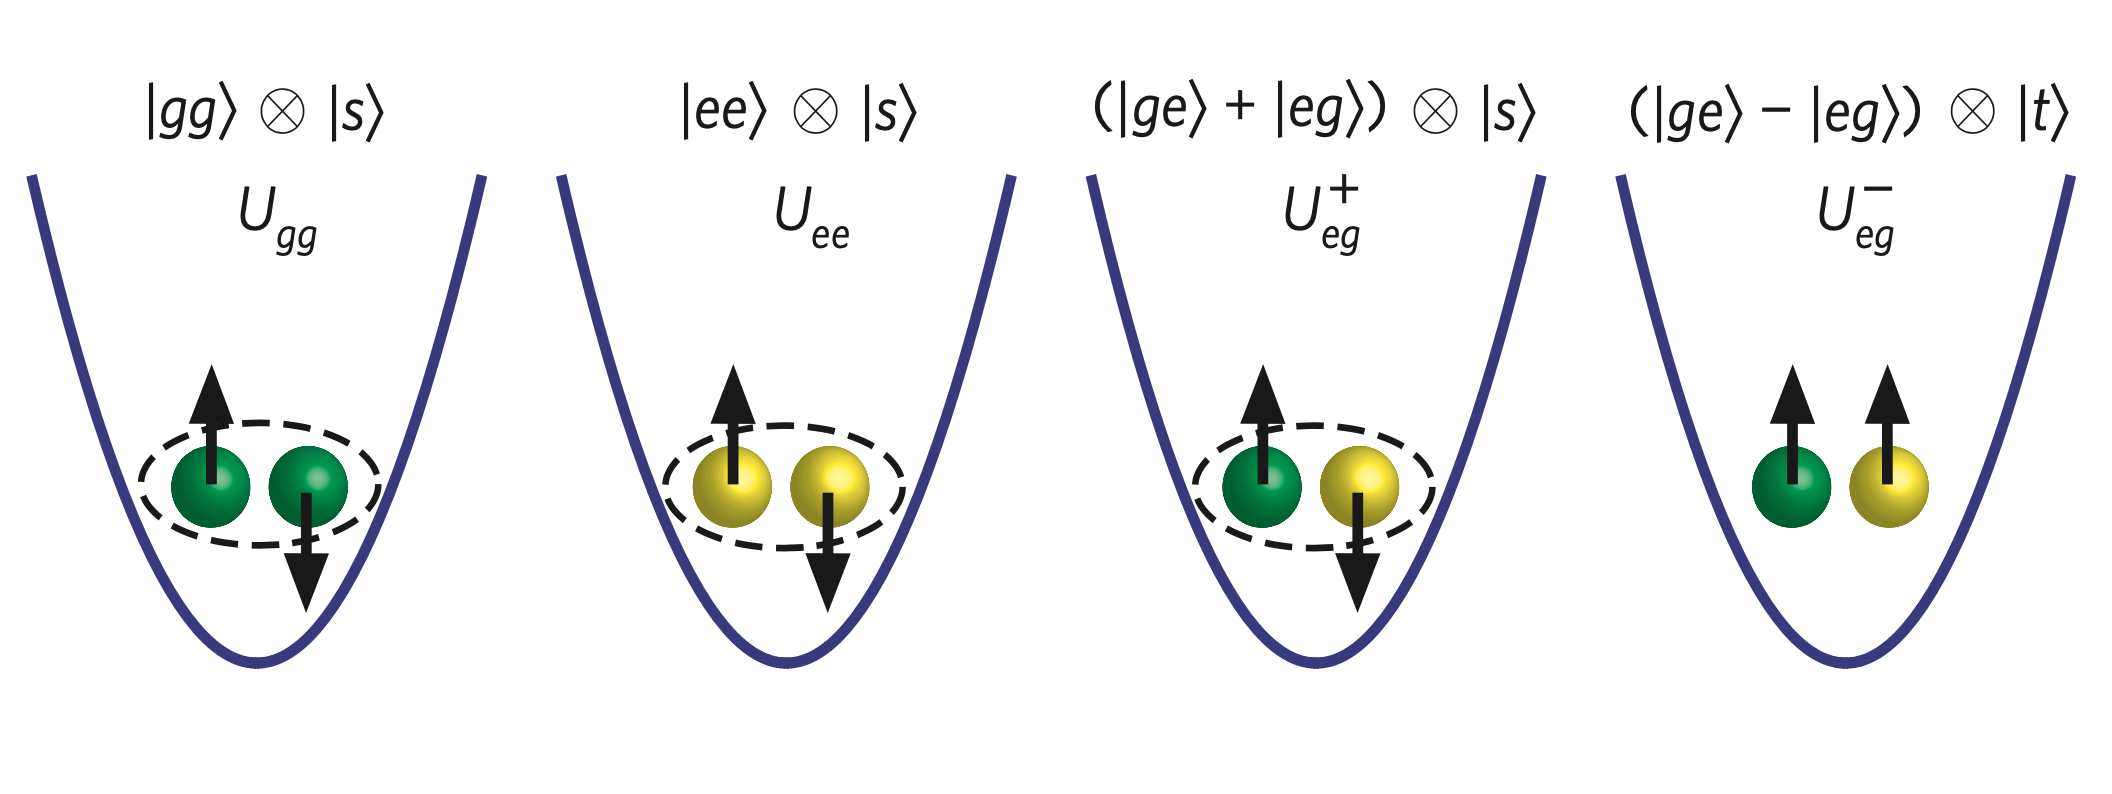
\includegraphics[width=0.7\textwidth]{eg.png}
    \bicaption{光晶格中四个散射通道。摘自\cite{gorshkov2010two}}{Four scattering channels in optical lattice. Reprinted from \cite{gorshkov2010two}}
    \label{eg}
\end{figure}
%%%%%%%%%%%%%%%%%%%%%%%%%%%%%%%%%%%%%%%%%%%%%%%%%%%%%%%%%%%%%%%%%%%%%%%%%%
\end{comment}
如果将$\hat{\rho}_{eg^\pm}$展开,我们得到不同轨道原子间的相互作用$\hat{V}_{eg}$分成了自旋交换与自旋守恒的两项:
\begin{equation}
\begin{aligned}
\hat{V}_{eg^+} &= g_{e g^+} \int \mathrm{d}^{3} \Vector{r} \hat{\rho}_{eg^+}(\Vector{r}) \hat{\rho}_{eg^+}(\Vector{r})+g_{e g^-} \int \mathrm{d}^{3} \Vector{r} \hat{\rho}_{eg^-}(\Vector{r}) \hat{\rho}_{eg^-}(\Vector{r})\\
\quad &= \frac{g_{e g}^{+}+g_{e g}^{-}}{2} \int \mathrm{d}^{3} \Vector{r} \rho_{e}(\Vector{r}) \rho_{g}(\Vector{r}) \\ 
&\quad \quad + \frac{g_{e g}^{+}-g_{e g}^{-}}{2} \sum_{m m^{\prime}} \int \mathrm{d}^{3} \Vector{r} \Psi_{g m}^{\dagger}(\Vector{r}) \Psi_{e m^{\prime}}^{\dagger}(\Vector{r}) \Psi_{g m^{\prime}}(\Vector{r}) \Psi_{e m}(\Vector{r})
\end{aligned}
\end{equation}
最后,将整个二次量子化哈密顿量在光晶格紧束缚近似下写为:
\begin{equation}
\begin{aligned}
\hat{H}=&-\sum_{\langle j, i\rangle \alpha, m} J_{\alpha}\left(c_{i \alpha m}^{\dagger} c_{j \alpha m}+\text { h.c. }\right)+\sum_{j, \alpha} \frac{U_{\alpha \alpha}}{2} n_{j \alpha}\left(n_{j \alpha}-1\right) \\
&+V \sum_{j} n_{j e} n_{j g}+V_{e x} \sum_{j, m, m^{\prime}} c_{j g m}^{\dagger} c_{j e m^{\prime}}^{\dagger} c_{j g m^{\prime}} c_{j e m}
\end{aligned}
\end{equation}
其中$\hat{n}_{j\alpha}=\sum_m \hat{n}_{j\alpha m}$,$V=\left(U_{e g}^{+}+U_{e g}^{-}\right) / 2$与$V_{ex}=\left(U_{e g}^{+}-U_{e g}^{-}\right) / 2$分别描述不同轨道原子间的自旋不变与自旋交换相互作用,其中:
\begin{equation}
U_{eg^\pm} = g_{eg^\pm} \int \mathrm{d}^{3} \Vector{r} w_e^2(\Vector{r})w_g^2(\Vector{r})
\end{equation}
有了上述丰富的轨道间相互作用与核自旋SU(N)自由度,这一模型可以用来模拟众多凝聚态物理中强关联多体模型,比如近藤晶格模型、自旋链模型、自旋液体等。

紧接着于2014年,Scazza F\cite{scazza2014observation}与合作者一起在${}^{173}$Yb体系中证实了上述自旋交换相互作用的存在。其思路如图~\ref{egexp}~所示:
%%%%%%%%%%%%%%%%%%%%%%%%%%%%%%%%%%%%%%%%%%%%%%%%%%%%%%%%%%%%%%%%%%%%%%%%%%
\begin{figure}[!htbp]
    \centering
    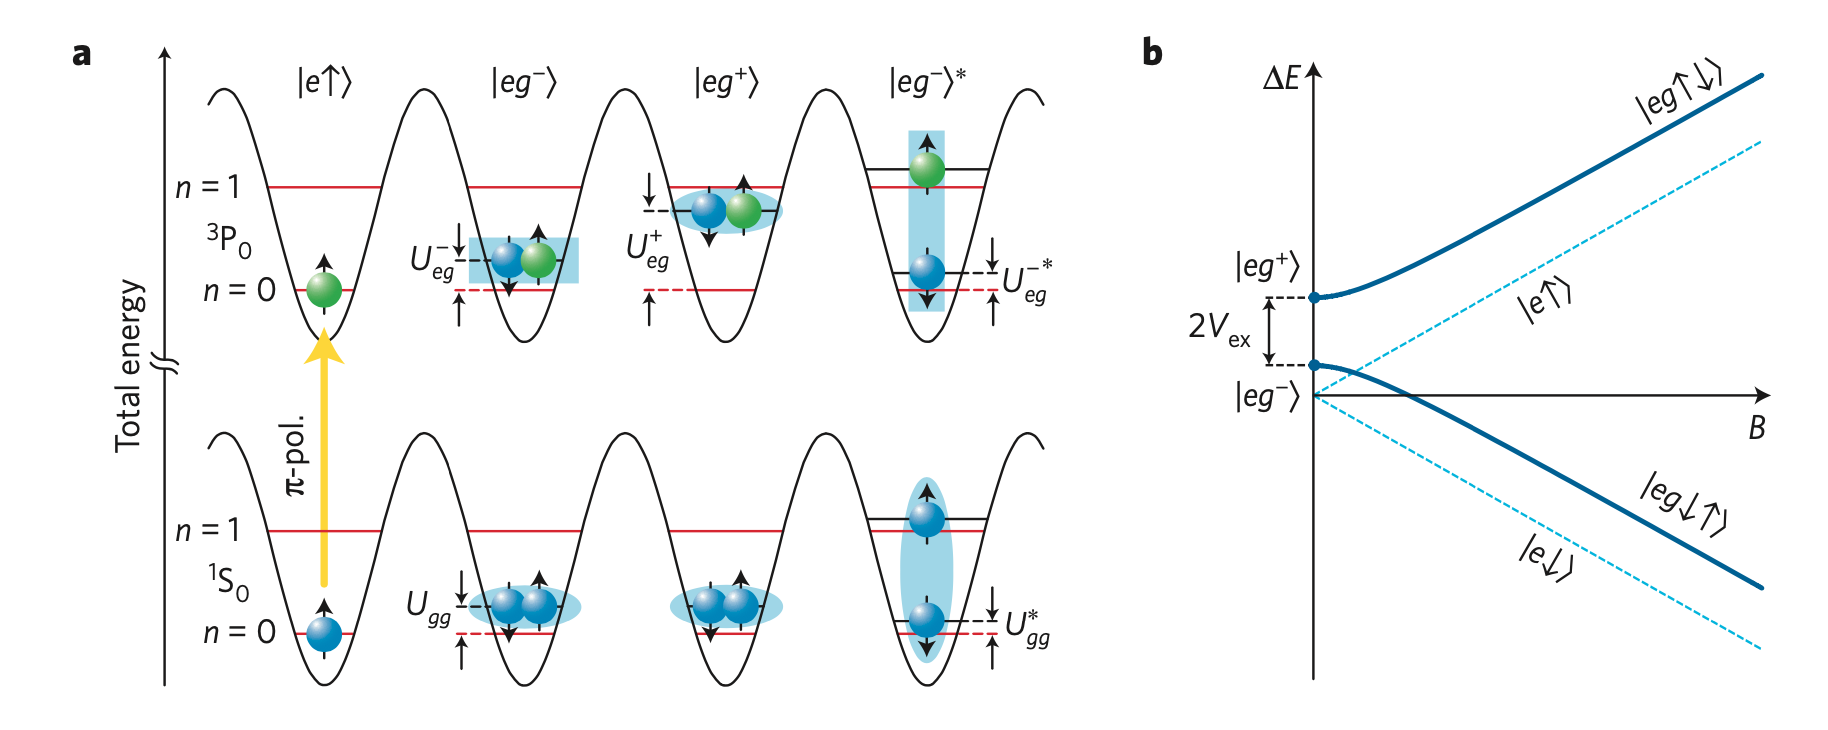
\includegraphics[width=0.7\textwidth]{./intro/egexp.png}
    \bicaption{自旋交换相互作用体系探测。图a代表单原子与双原子初态到末态的跃迁。图b代表末态的能谱。摘自\citep{scazza2014observation}}{Detection of spin-exchange system. Fig a for transition from initial state to final state under laser field. Fig b for energy spectrum of final state. Reprinted from \citep{scazza2014observation}}
    \label{egexp}
\end{figure}
%%%%%%%%%%%%%%%%%%%%%%%%%%%%%%%%%%%%%%%%%%%%%%%%%%%%%%%%%%%%%%%%%%%%%%%%%%
该实验选取不同电子排布($g({}^1S_0)$与$e({}^3P_0)$)的${}^{173}$Yb($I=5/2$)原子,束缚在较深(原子不能自由移动)的光晶格中,在每个格点里面,原子间的相互作用能为:
\begin{equation}
U_{X}=\frac{4 \pi \hbar^{2}}{m} a_{X} \int \mathrm{d}^{3} r w_{a}^{2}(\Vector{r}) w_{b}^{2}(\Vector{r})
\end{equation}
其中$X =gg, ee, eg^+, eg^−$代表不同状态的原子对。装载不同核自旋的$g$轨道原子到光晶格中,平均填充在$\bar{n}=1$与$\bar{n}=2$之间,这样导致部分格点内有一个原子,部分格点内有两个原子。对于有两个原子的格点,用激光将一个原子从g态激发到e态,末态有两个本征态$|eg^\pm\rangle$,本征能量为$U_{eg^\pm}$。如果在体系中加入沿$z$方向的磁场,导致$|eg^\pm\rangle$两态之间有非零的跃迁矩阵元,最终的哈密顿量为:
\begin{equation}
\hat{H}_{eg}=\left(\begin{array}{cc}
U_{e g}^{+} & \Delta_{B} \\
\Delta_{B} & U_{e g}^{-}
\end{array}\right)
\end{equation}
其中$\Delta_{B}=\delta g m_{\mathrm{F}} \mu_{\mathrm{B}} B$,$\delta g$为核自旋朗德因子的差值,跃迁末态的本征能量为:
\begin{equation}
E_{1,2}=V \pm \sqrt{V_{\mathrm{ex}}^{2}+\Delta_{B}^{2}}
\end{equation}
本征波函数为$|eg^\pm\rangle$两态的线性叠加。

\begin{comment}
如图~\ref{egd}~
%%%%%%%%%%%%%%%%%%%%%%%%%%%%%%%%%%%%%%%%%%%%%%%%%%%%%%%%%%%%%%%%%%%%%%%%%%
\begin{figure}[!htbp]
    \centering
    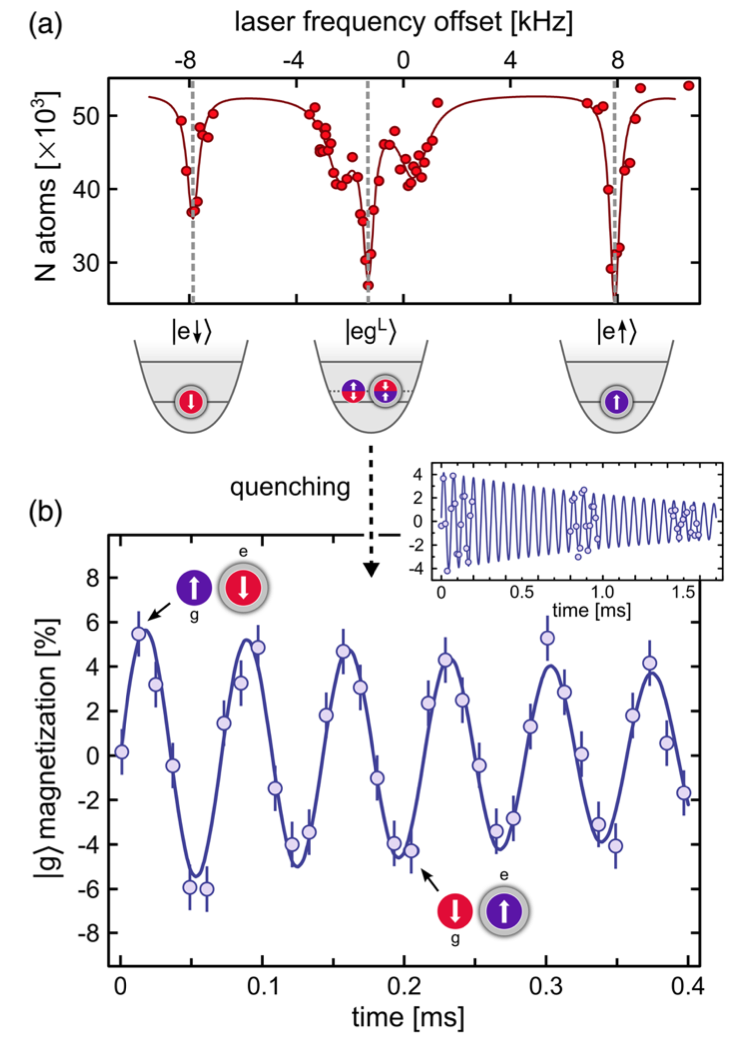
\includegraphics[width=0.6\textwidth]{chap1spexd.png}
    \bicaption{图a代表实验测到的吸收谱,不同的峰代表了不同的末态。图b代表观测到自旋交换体系的的自旋动力学。摘自\citep{cappellini2014direct}}{Fig(A) for spectrum of clock transition. Fig(B) for time resolved spin transition. dynamics. Reprinted from \citep{cappellini2014direct}}
    \label{egd}
\end{figure}
%%%%%%%%%%%%%%%%%%%%%%%%%%%%%%%%%%%%%%%%%%%%%%%%%%%%%%%%%%%%%%%%%%%%%%%%%%
\end{comment}

通过观测不同磁场下的共振谱,得到不同磁场下末态的能量。进一步地,研究者通过测量初态自旋分布到末态自旋分布演化\cite{scazza2014observation,cappellini2014direct},直接观测到了自旋交换相互作用。拟合实验中不同磁场下测到的共振峰的位置,最终测到${}^{173}$Yb原子间裸的散射长度为\cite{scazza2014observation,cappellini2014direct}:
\begin{equation}
\begin{split}
a_{e g}^{-}&=(3300 \pm 300) a_{0}\\
a_{e g}^{+}& = 219.5 a_0\\
\end{split}
\end{equation}
可以看到为铁磁耦合。与此同时,研究者也观测到了Sr原子体系的铁磁自旋交换相互作用\cite{zhang2014spectroscopic}。

但是上述观测到的裸的原子间相互作用为铁磁自旋耦合,模拟近藤物理需要反铁磁耦合。这时候理论研究者提出利用束缚诱导共振来调节,一系列系统的工作表明利用束缚诱导共振来调节反铁磁自旋交换的强度\cite{zhang2016kondo,cheng2017enhancing,zhang2018control,ji2018confinement,zhang2020tight,zhang2020controlling}。最终实验上成功观测到了的准一维体系束缚诱导增强的自旋动力学\cite{riegger2018localized}。如图~\ref{CIRspexexp}~所示。
%%%%%%%%%%%%%%%%%%%%%%%%%%%%%%%%%%%%%%%%%%%%%%%%%%%%%%%%%%%%%%%%%%%%%%%%%%
\begin{figure}[!htbp]
    \centering
    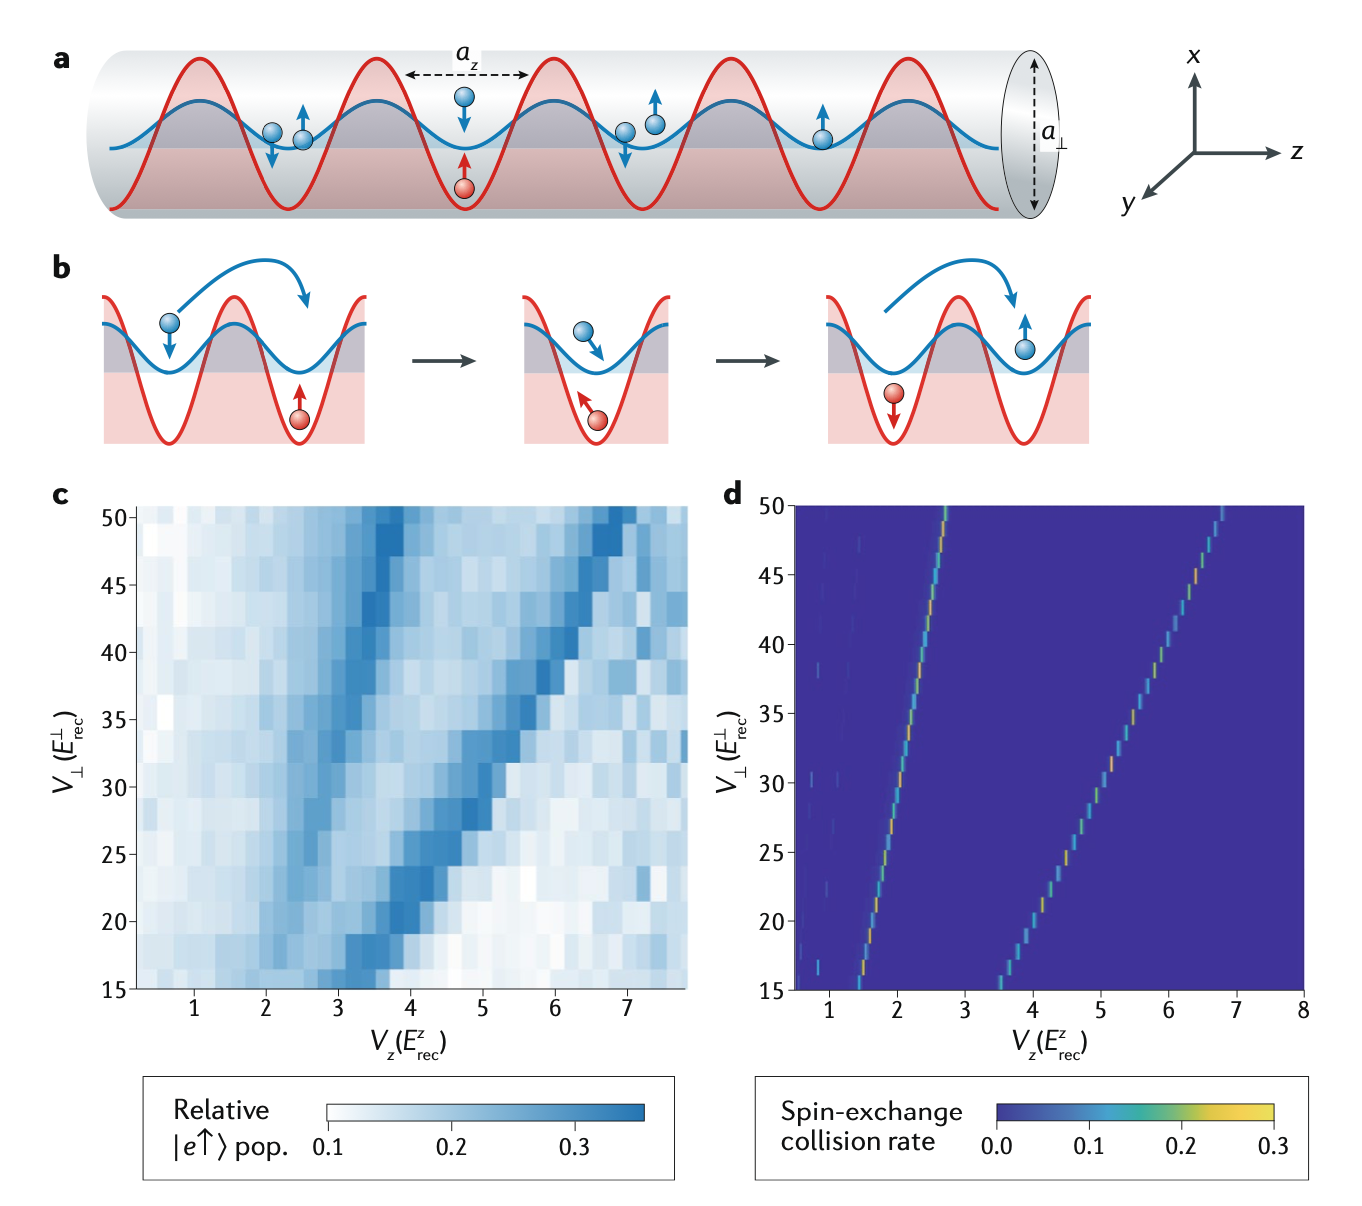
\includegraphics[width=0.7\textwidth]{./intro/chap1spexCIR.png}
    \bicaption{束缚诱导共振调节的自旋交换相互作用。图a代表准一维体系z方向上自旋相关的晶格制造巡游费米子与局域费米子。图b代表自旋交换发生的过程。图c,d分别代表实验测量与理论预测的束缚诱导增强下的自旋交换动力学。摘自\citep{riegger2018localized,zhang2020controlling}}{ Tunable spin-exchange interaction by confinement induced resonance. Fig a for quasi 1D system, which consists of spin-dependent lattice to creat free hopping fermions and localized spin. Fig b for illustration of spin exchange process. Fig c and d for Experimental and theoretical spin exchange interaction enchanced by confinement induced resonance. Reprinted from \citep{riegger2018localized,zhang2020controlling}}
    \label{CIRspexexp}
\end{figure}
%%%%%%%%%%%%%%%%%%%%%%%%%%%%%%%%%%%%%%%%%%%%%%%%%%%%%%%%%%%%%%%%%%%%%%%%%%












\section{费米极化子物理}\label{1sec:polaron}
极化子是一个杂质物理中比较古老的概念。早在固体物理中就有研究大极化子与小极化子\cite{landau1933bewegung,pekar1946autolocalization,frohlich1950xx,frohlich1954electrons,feynman1955slow,mahanmany},对应的是电子在晶格中运动,电子的单粒子性质被晶格声子激发所修饰,改变其有效质量、寿命等。严格说晶格里的极化子属于玻色极化子。如果将背景原子改为多体费米体系,就得到费米极化子。近年来,随着冷原子中密度不均衡费米混合气体的制备,费米极化子作为其中的极端体系,进入研究者的视野,结合冷原子体系特有的控制、操控、观测能力,极化子的研究迎来新的阶段,我们将围绕相关研究的实验与理论展开。

费米极化子是典型的费米液体,冷原子物理中Feshbach可调节相互作用带来了对整个相互作用区间的关注。冷原子中费米极化子的研究最早可追溯到Chevy变分波函数\cite{chevy2006},这是个典型的N+1体系。系统哈密顿量为:
\begin{equation}
\hat{H}=\sum_{k, \sigma} \epsilon_{k} \hat{a}_{k, \sigma}^{\dagger} \hat{a}_{k, \sigma}+\frac{g_{b}}{V_{k, \boldsymbol{k}^{\prime}, q}} \sum_{\boldsymbol{k}+q, 1}^{\dagger} \hat{a}_{\boldsymbol{k}^{\prime}-q, 2}^{\dagger} \hat{a}_{\boldsymbol{k}^{\prime}, 2} \hat{a}_{\boldsymbol{k}, 1}
\end{equation}
采用Chevy变分波函数:
\begin{equation}
\left|\psi_{0}\right\rangle=\left(\phi_{0} d_{\Vector{0}}^{\dagger}+\sum_{\Vector{k}, \Vector{q}}^{\prime} \phi_{\Vector{k q}} d_{\Vector{q}-\Vector{k}}^{\dagger} u_{\Vector{k}}^{\dagger} u_{\Vector{q}}\right)\left|\mathrm{FS}_{\uparrow}^{N}\right\rangle
\end{equation}
带入到薛定谔方程中得到:
\begin{equation}
\begin{split}
&\left(\epsilon_{k}+\epsilon_{q-k}-\epsilon_{q}\right) \phi_{k, q}+\frac{g_{b}}{V} \sum_{k^{\prime}} \phi_{k^{\prime}, q}+\frac{g_{b}}{V} \phi_{0}=E \phi_{k, q}\\
&\frac{g_{b}}{V} \sum_{q} \phi_{0}+\frac{g_{b}}{V} \sum_{q, k} \phi_{k, q}=E \phi_{0}\\
\end{split}
\end{equation}
引入辅助变量$\chi(\boldsymbol{q})=\phi_{0}+\sum_{\boldsymbol{k}} \phi_{k, \boldsymbol{q}}$得到能量满足自洽方程:
\begin{equation}
E=\sum_{q<k_{F}} \frac{1}{\sum_{k>k_{F}}\left(\frac{1}{\epsilon_{\boldsymbol{k}}+\epsilon_{q-k}-\epsilon_{q}-E}-\frac{1}{2 \epsilon_{\boldsymbol{k}}}\right)-\sum_{k<k_{F}} \frac{1}{2 \epsilon_{k}}} \label{consistentEQ}
\end{equation}
%%%%%%%%%%%%%%%%%%%%%%%%%%%%%%%%%%%%%%%%%%%%%%%%%%%%%%%%%%%%%%%%%%%%%%%%%%
\begin{figure}[!htbp]
    \centering
    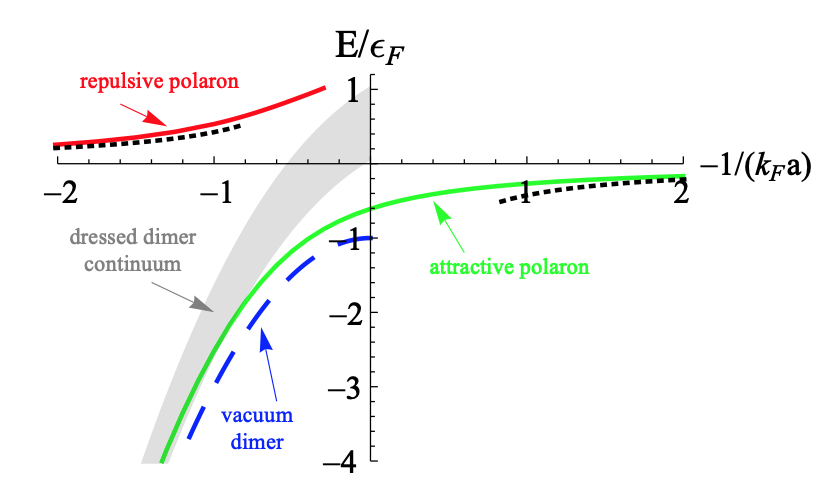
\includegraphics[width=0.7\textwidth]{./intro/chap1fpspectrum.png}
    \bicaption{单粒子空穴近似下的吸引极化子与排斥极化子能量。绿色对应吸引极化子,红色对应排斥极化子的解,中间灰色区域对应分子态。摘自\citep{massignan2014polarons}}{Energy of attractive and repulsive fermi polarons under 1 p-h approximation. Green line for attractive polaron, red line for repulsive polarons and gray area for continuous dreesed molecules.  Reprinted from\citep{massignan2014polarons}}
    \label{fpchevyE}
\end{figure}
%%%%%%%%%%%%%%%%%%%%%%%%%%%%%%%%%%%%%%%%%%%%%%%%%%%%%%%%%%%%%%%%%%%%%%%%%%
求解最低能量可以得到吸引极化子,如图~\ref{fpchevyE}~所示。在弱相互作用区间,基态为极化子态,本征能量为$E_-$,在BCS极限下$E_{-}=2 \pi a n_{\uparrow} / m_{r}$。随着相互作用增强,杂质原子与背景费米海中任意位置的一个原子配对形成分子,带来一段连续能谱区间,宽度大约为$E_F$,其中零动量分子的能量可以利
用新的分子态变分波函数\cite{Mora_pm,Punk_pm,combescot2010analytical,Trefzger2012Impurity}来得到:
\begin{equation}
\left|\psi_{1}\right\rangle=\left(\sum_{\Vector{k}}^{\prime} \xi_{\Vector{k}} d_{-\Vector{k}}^{\dagger} u_{\Vector{k}}^{\dagger}+\sum_{\Vector{k}^{\prime}, \Vector{k}, \Vector{q}}{ }^{\prime} \xi_{\Vector{k}^{\prime} \Vector{k q}} d_{\Vector{q}-\Vector{k}-\Vector{k}^{\prime}}^{\dagger} u_{\Vector{k}^{\prime}}^{\dagger} u_{\Vector{k}}^{\dagger} u_{\Vector{q}}\right)\left|\mathrm{FS}_{\uparrow}^{N-1}\right\rangle
\end{equation}
求得一支被费米海修饰的分子态的能量解,与极化子能量比较可以发现转变点在$1/k_Fa_S=0.84$,如图~\ref{pmE}~所示:
%%%%%%%%%%%%%%%%%%%%%%%%%%%%%%%%%%%%%%%%%%%%%%%%%%%%%%%%%%%%%%%%%%%%%%%%%%
\begin{figure}[!htbp]
    \centering
    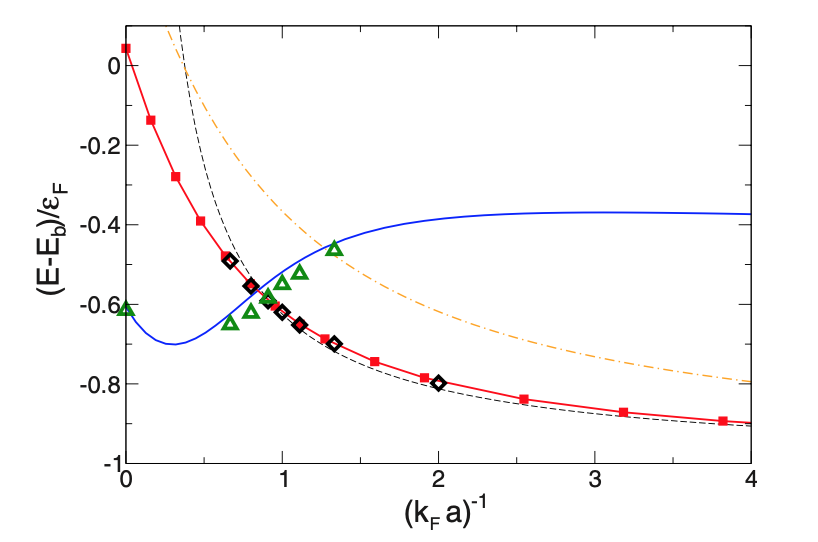
\includegraphics[width=0.7\textwidth]{./intro/chap1pmE.png}
    \bicaption{极化子-分子转变。其中蓝色实线代表一对粒子-空穴激发近似下的零动量极化子。红色实线代表考虑一对粒子空穴激发修饰的分子能量,橘黄色虚线代表费米面存在裸的分子态能量。散点为蒙特卡洛的结果。摘自\citep{Punk_pm}}{Polaron-molecule transition. Blue solid line for zero momentum attractive polaron branch under 1 p-h excitation approximation, red solid line for dreesed molecule under 1 p-h excitation approximation, yellow dashed line for bare molecule with fermi sea. Scatterd points for result from MC. Reprinted from\citep{Punk_pm}}
    \label{pmE}
\end{figure}
%%%%%%%%%%%%%%%%%%%%%%%%%%%%%%%%%%%%%%%%%%%%%%%%%%%%%%%%%%%%%%%%%%%%%%%%%%
极化子到分子的转变除了上述变分方法的研究之外,利用量子蒙特卡罗算法也可以研究极化子体系。最早在极化气体中利用Fixed-node蒙卡算法可以求得低杂质密度下费米液体行为\cite{Pilati2008phase}。 利用图蒙卡可以得到转变点为$1/k_Fa_S=0.9$,相应地极化子与分子的单粒子性质比如有效质量在转变点附近发散,如图~\ref{MCeffectm}~所示。极化子的准粒子剩余等也可以由蒙卡方法得到\cite{Prokoffermi,Prokofbold,VlietinckMC}。
%%%%%%%%%%%%%%%%%%%%%%%%%%%%%%%%%%%%%%%%%%%%%%%%%%%%%%%%%%%%%%%%%%%%%%%%%%
\begin{figure}[!htbp]
    \centering
    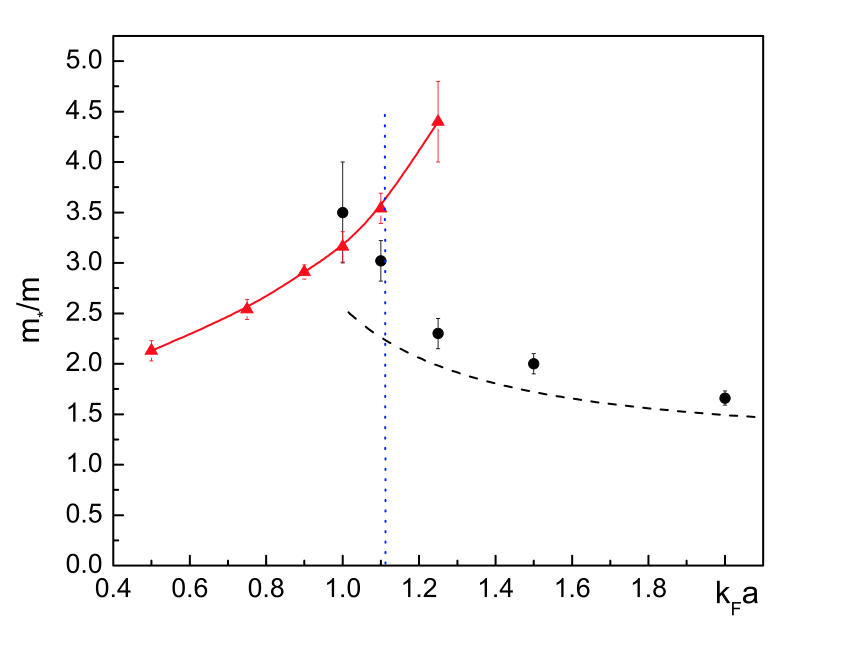
\includegraphics[width=0.7\textwidth]{./intro/chap1MCeffectm.png}
    \bicaption{极化子-分子转变附近极化子与分子的有效质量。其中红色点对应分子有效质量,黑色点对应吸引极化子有限质量,蓝色虚线对应1p-h近似下的转变点。摘自\citep{Prokoffermi}}{Effective mass of polaron and molecule near polaron-molecule transition. Red points for molecule. Black points for polaron. Blue dashed line for polaron-molecule transition point under 1 p-h approximation. Reprinted from\citep{Prokoffermi}}
    \label{MCeffectm}
\end{figure}
%%%%%%%%%%%%%%%%%%%%%%%%%%%%%%%%%%%%%%%%%%%%%%%%%%%%%%%%%%%%%%%%%%%%%%%%%%

在强相互作用区间,远离基态还可以求得方程~\ref{consistentEQ}~一支$E_+>0$的激发态解,随着杂质原子间的相互作用越过共振点,从低能有效散射角度来看杂质原子与背景之间为有效的互相排斥,被称为排斥极化子\cite{Cui2010Stability},在少体物理中对应upper branch,在BEC极限下,我们有$E_{+}=2 \pi a n_{\uparrow} / m_{r}$。

另一方面采用T矩阵单粒子空穴激发近似,计算杂质原子自能也可以得到上述变分波函数相同的自洽方程\cite{Combescot20071ph},令人惊讶的是这样简单的单粒子空穴近似在共振处依然可以成立,其背后的原因在于高阶粒子空穴激发的抵消作用\cite{Combescot20071ph008full}。
%%%%%%%%%%%%%%%%%%%%%%%%%%%%%%%%%%%%%%%%%%%%%%%%%%%%%%%%%%%%%%%%%%%%%%%%%%
\begin{figure}[!htbp]
    \centering
    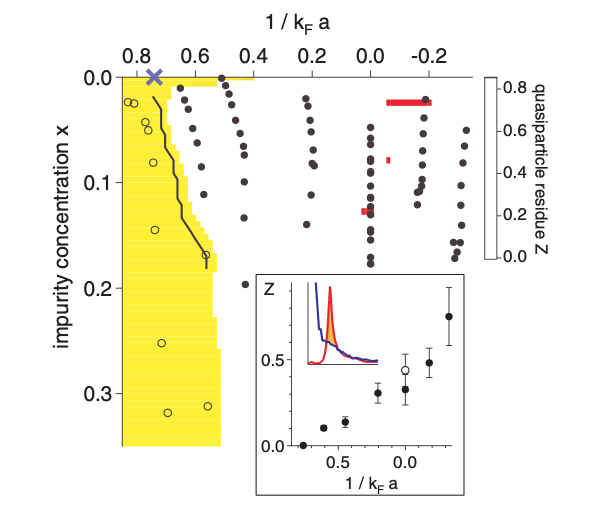
\includegraphics[width=0.6\textwidth]{./intro/chap1fpZ.png}
    \bicaption{准粒子剩余随着相互作用与密度的变化。摘自\citep{Schirotzekobservation}}{Quasiparticle residue as a function of interaction and impurity densuty. Reprinted from \citep{Schirotzekobservation}}
    \label{fpZ}
\end{figure}
%%%%%%%%%%%%%%%%%%%%%%%%%%%%%%%%%%%%%%%%%%%%%%%%%%%%%%%%%%%%%%%%%%%%%%%%%%
实验中费米极化子在非均衡密度的混合费米气体中首先被观测到。其中少数原子成为杂质,多数原子构成背景。杂质原子的单粒子性质被背景费米海上的粒子-空穴激发所重整化。

费米极化子最早的直接实验证据来自MIT研究组\cite{Schirotzekobservation}。实验上制备含有$10^6$个$|1\rangle{}^6$Li原子的体系。然后通过双光子过程将大约$2\%$的$|1\rangle$原子激发到$|3\rangle$。调节$|1\rangle$与$|2\rangle$之间的相互作用,然后通过测量$3|\rangle$到$|2\rangle$的rf谱,通过谱峰的位置来给出极化子的能量,

\begin{comment}
如图~\ref{fpE}~所示。
%%%%%%%%%%%%%%%%%%%%%%%%%%%%%%%%%%%%%%%%%%%%%%%%%%%%%%%%%%%%%%%%%%%%%%%%%%
\begin{figure}[!htbp]
    \centering
    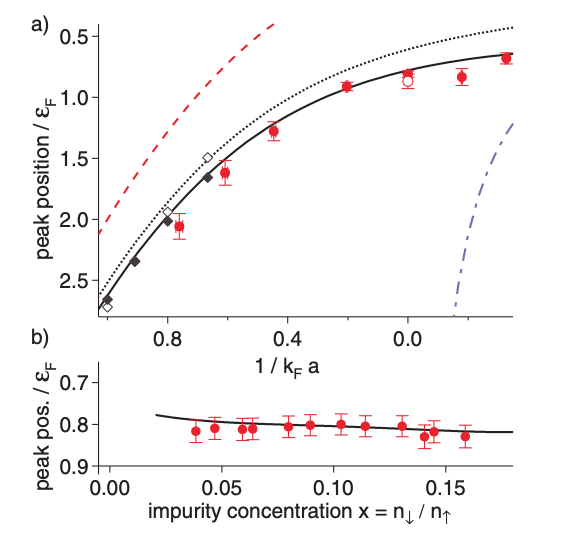
\includegraphics[width=0.7\textwidth]{chap1fpE.png}
    \bicaption{图a为实验测到的(散点)以及理论预测(黑色实线)的费米极化子能量随相互作用变化曲线。图b为rf谱峰的位置随杂质密度的变化。摘自\citep{Schirotzekobservation}}{Fig(a) for measured and predicted energy of fermi polaron upon interaction. Fig(b) for rf spectrum peak position upon impurity densuty. Reprinted from\citep{Schirotzekobservation}}
    \label{fpE}
\end{figure}
%%%%%%%%%%%%%%%%%%%%%%%%%%%%%%%%%%%%%%%%%%%%%%%%%%%%%%%%%%%%%%%%%%%%%%%%%%
可以看到,即使在共振点处,理论计算的能量与实验测到的能量也符合很好。并且谱峰的位置受杂质密度变化影响较小,处于低密度区间。
\end{comment}

分析射频谱的面积,提取出准粒子剩余,如图~\ref{fpZ}~所示,可以看到越过一个临界相互作用,准粒子留数降到了零。这意味着当相互作用越过共振点,极化子能量越来越低,完成基态从极化子到分子的转变。
%%%%%%%%%%%%%%%%%%%%%%%%%%%%%%%%%%%%%%%%%%%%%%%%%%%%%%%%%%%%%%%%%%%%%%%%%%
\begin{figure}[!htbp]
    \centering
    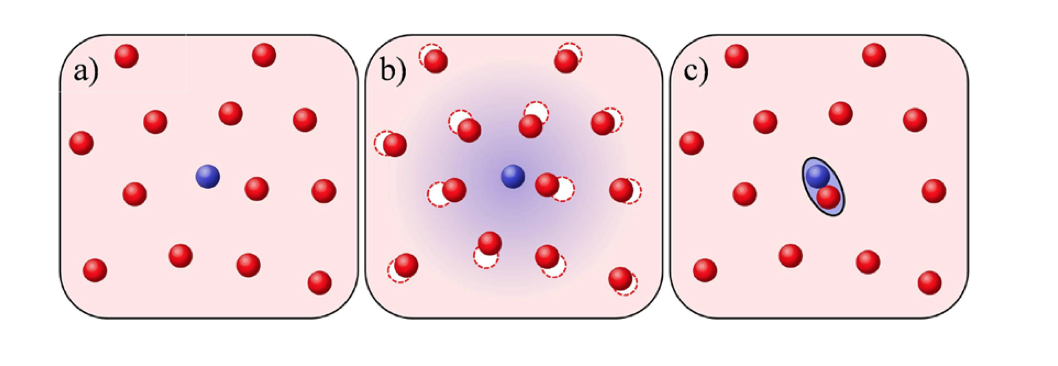
\includegraphics[width=0.7\textwidth]{./intro/chap1fp.png}
    \bicaption{费米极化子到分子转变的示意图。相互作用从弱变强依次从极化子变到分子。摘自\citep{Schirotzekobservation}}{Illustration of transition from Fermi polaron to molecule. As interaction goes strong, impurity goes from polaron to molecule. Reprinted from \citep{Schirotzekobservation}.}
    \label{fp}
\end{figure}
%%%%%%%%%%%%%%%%%%%%%%%%%%%%%%%%%%%%%%%%%%%%%%%%%%%%%%%%%%%%%%%%%%%%%%%%%%
进一步实验\cite{kohstall2012metastability}采用不同的体系,制备少量${}^{40}$K与大量${}^{6}$Li的混合气,通过射频脉冲将与Li原子无相互作用的$|0\rangle\equiv\left|F=9 / 2, m_{\mathrm{F}}=-7 / 2\right\rangle$激发到与Li原子有Feshbach共振调节相互作用的$|1\rangle \equiv\left|F=9 / 2, m_{\mathrm{F}}=-5 / 2\right\rangle$。观测到在吸引极化子之上的排斥极化子,如图~\ref{upfp}~所示 :
%%%%%%%%%%%%%%%%%%%%%%%%%%%%%%%%%%%%%%%%%%%%%%%%%%%%%%%%%%%%%%%%%%%%%%%%%%
\begin{figure}[!htbp]
    \centering
    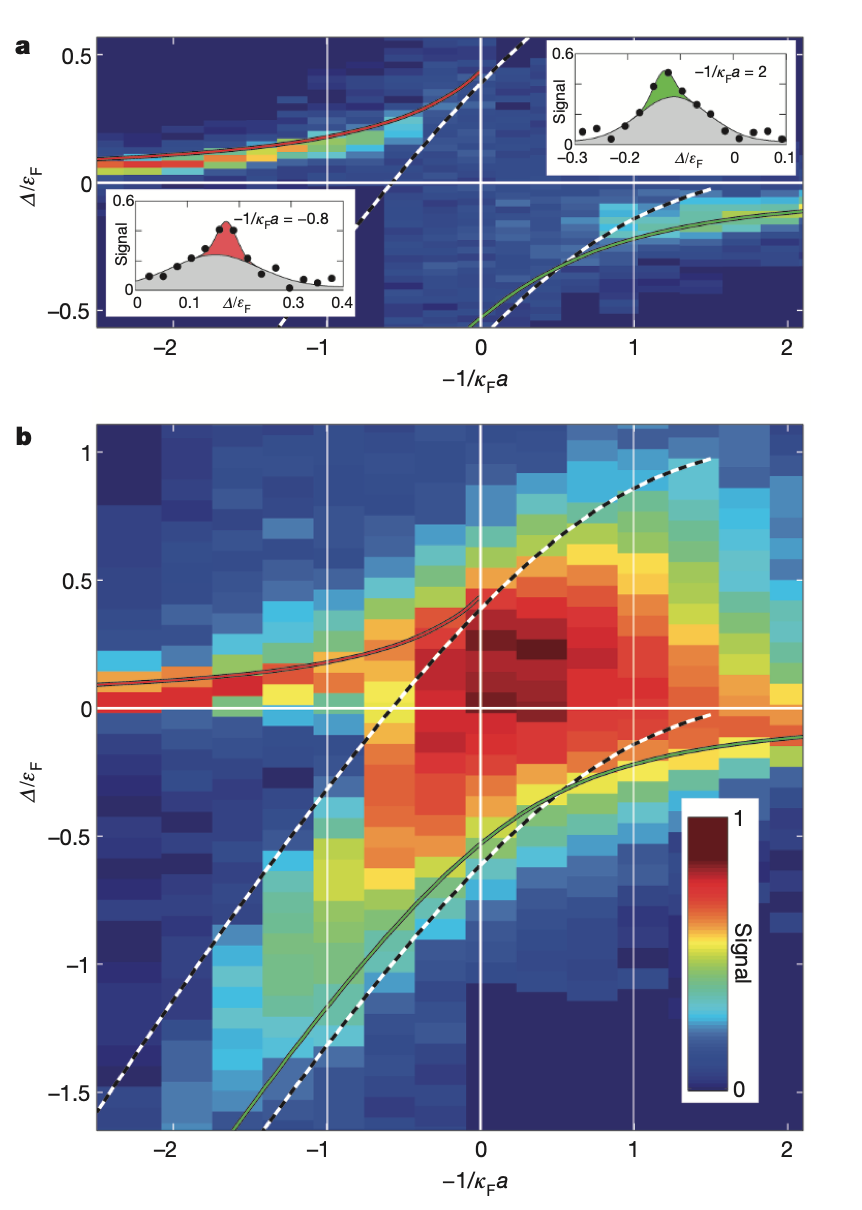
\includegraphics[width=0.6\textwidth]{./intro/chap1upfp.png}
    \bicaption{ 极化子测量得到的射频谱。图a(弱)与b(强)为不同rf场强下测到的吸收谱。可以清楚地看到吸引极化子与排斥极化子两支解,在中间伴有分子态。\citep{kohstall2012metastability}}{Rf spectrum of polaron. Fig a and Fig b for transition spectrum measured under weak and strong rf power. There are attractive polaron branch, repulsive polaron branch ang molecule branch. Reprinted from \citep{kohstall2012metastability}}
    \label{upfp}
\end{figure}
%%%%%%%%%%%%%%%%%%%%%%%%%%%%%%%%%%%%%%%%%%%%%%%%%%%%%%%%%%%%%%%%%%%%%%%%%%
后续在纯${}^{6}$Li体系中也观测到了排斥极化子\cite{Scazzarepulsive}。

\begin{comment}
后续对于排斥极化子对应的极化气体中的铁磁关联也有一定的量子蒙特卡罗数值研究\cite{Conduit2009Inhomo,Pilati2010Itinerant,chang2011ferromagnetism}。除了蒙特卡罗数值以外,通过泛函重整化群也可以得到吸引极化子和排斥极化子的谱密度\cite{Schmidt2011excitation}。

我们知道在低维体系中密度涨落会扮演更重要的角色。那对于二维体系的费米极化子会是如何呢?研究者在${}^{40}$K二维光晶格中实现了二维费米极化子,并观测到了吸引与排斥极化子\cite{koschorreck2012attractive}。
%%%%%%%%%%%%%%%%%%%%%%%%%%%%%%%%%%%%%%%%%%%%%%%%%%%%%%%%%%%%%%%%%%%%%%%%%%
\begin{figure}[!htbp]
    \centering
    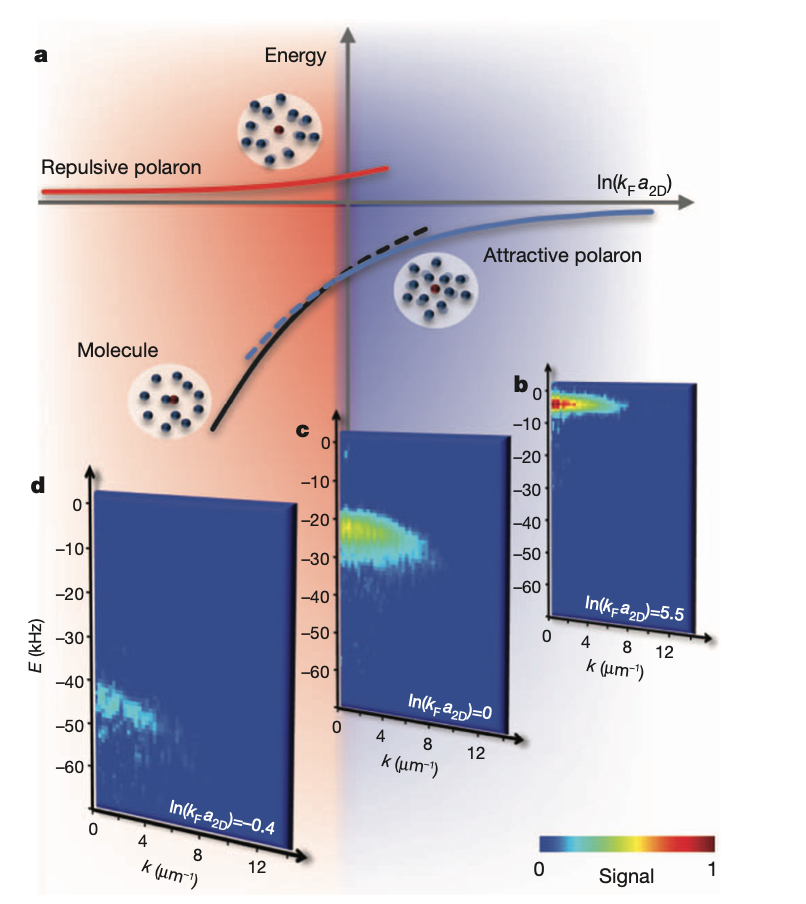
\includegraphics[width=0.7\textwidth]{./intro/chap12dfp.png}
    \bicaption{二维极化子实验观测。排斥极化子、吸引极化子、分子态均被观测到。摘自\citep{koschorreck2012attractive} }{Fermi polaron in 2D, with repulsive branch, attractive branch and molecule. Reprinted from \citep{koschorreck2012attractive} }
    \label{2dfp}
\end{figure}
%%%%%%%%%%%%%%%%%%%%%%%%%%%%%%%%%%%%%%%%%%%%%%%%%%%%%%%%%%%%%%%%%%%%%%%%%%
随着实验技术的成熟,对于极化子探索的方向也有所扩展。比如利用Ramesy相干动力学来研究\cite{Cetina2015decoherence,cetina2016ultrafast}极化子的形成、有限温度下的极化子准粒子性质的破坏\cite{YanBoiling}、以及利用轨道Feshbach共振来调节的极化子等\cite{Darkwah2019}。

%通过改变杂质原子与背景费米子的质量比,我们还可以观察到三聚体的形成\cite{Mathy2011trimers}

在费米极化子实验测量中,最常用的测量手段是rf谱测量。理论上rf谱相应的计算最早来自\cite{Massignan2008Twin},其原理可用简单的三态模型来阐述,制备少量$|1\rangle$态原子与背景$|2\rangle$态原子,之间的相互作用可以调节。然后用rf脉冲将一部分$|1\rangle$态激发到与1,2体系没有相互作用的$|0\rangle$态,rf激发场的哈密顿量为:
\begin{equation}
H_{\mathrm{rf}}=\frac{\Omega}{2} \int \mathrm{d}^{3} r\left[\mathrm{e}^{-\mathrm{i} \omega t} \psi_{1}^{\dagger}(\boldsymbol{r}, t) \psi_{0}(\boldsymbol{r}, t)+\text { h.c. }\right]
\end{equation}
在$|1\rangle$态原子数目很小的情况下,线性响应理论成立,rf场诱导的转化几率随频率变化$R(\omega)$:
\begin{equation}
R(\omega) \propto-\operatorname{Im} \mathcal{D}(\omega) \equiv-\int \mathrm{d}^{3} r \mathrm{~d}^{3} r^{\prime} \operatorname{Im} \mathcal{D}\left(\boldsymbol{r}, \boldsymbol{r}^{\prime}, \omega\right)
\end{equation}
其中$\mathcal{D}(\omega)$为推迟格林函数:
\begin{equation}
G(\boldsymbol{r},\boldsymbol{r}^{\prime},t,t^{\prime}) = -\mathrm{i} \theta\left(t-t^{\prime}\right)\left\langle\left[\psi_{1}^{\dagger}(\boldsymbol{r}, t) \psi_{0}(\boldsymbol{r}, t)\right.\right.\left.\left.\psi_{0}^{\dagger}\left(\boldsymbol{r}^{\prime}, t^{\prime}\right) \psi_{1}\left(\boldsymbol{r}^{\prime}, t^{\prime}\right)\right]\right\rangle
\end{equation}
的傅立叶变换。仅考虑1,2态原子存在相互作用的情况下,可以得到:
\begin{equation}
\begin{split}
&\operatorname{Im} \mathcal{D}(\omega)=-\frac{1}{2} \int \frac{\mathrm{d}^{3} k}{(2 \pi)^{3}} \int \frac{\mathrm{d} \epsilon}{2 \pi}[f(\epsilon)-f(\epsilon+\tilde{\omega})] \\
&\quad \times A_{0}(\boldsymbol{k}, \epsilon) A_{1}(\boldsymbol{k}, \epsilon+\tilde{\omega})
\end{split}
\end{equation}
其中$f(x)=[\exp (\beta x)+1]^{-1}$为费米分布。根据转变的方向可将rf谱分为两类:正向与逆向。初始态仅少量$|1\rangle$原子,rf场将与背景有相互作用的$|1\rangle$原子激发到与背景无相互作用的$|0\rangle$原子,此即正向rf谱。若初始态为少量$|0\rangle$
原子,rf场将与背景无相互作用的$|0\rangle$原子激发到与背景有相互作用的$|1\rangle$原子,此即逆向rf谱。逆向谱的优势在于可以测量整个频率区间的谱相应。

受到实验上对于费米极化子研究的拓展的启发,理论方面也扩展到关于动力学演化与有限温度下费米极化子的研究。基于实验上对Ramesy信号的测量,Parish利用截断粒子空穴的波函数方法\cite{Parish2016quantum}研究Ramesy信号。另一方面基于有限温度极化子实验的启发\cite{YanBoiling},吸引极化子、排斥极化子、分子极化子相变以及rf谱测量谱函数等概念在有限温度下的命运也得到了充分的理论研究,随着温度的升高,极化子的准粒子性质被破坏,相干性降低\cite{tajima2018many,Hu2018attractive,mulkerin2019breakdown,Taylor2019thermal,Liu2020Radio,Liu2020theory,Parish2021thermodynamic}。
\end{comment}

除了上述三维的研究之外,低维情况下的极化子也有很多研究,低维下涨落变得更加重要,任意吸引势下都会存在束缚态。在二维下与三维结论类似:极化子-分子转变依然被认为存在\cite{Zollner2011Polarons,Parish2011pm,Lewenstein2013spinchain012High}。吸引极化子与排斥极化子也存在\cite{Schmidt2012fermi,Ngampruetikorn_2012}。但是在一维下,N+1的体系存在贝特假设严格解\cite{mcguire1965interacting,mcguire1966interacting},变分波函数依然可以给出与贝特假设严格解一致的结果,即一维下不存在极化子到分子的转变\cite{Giraud2009highly,Leskinen_2010,Astrakharchik2013trapped}。

在极化子到分子的转变研究中,对于单极化子来说是个一阶转变。最近通过Raman光谱,研究者进一步揭示了存在有限密度和有限温度下极化子到分子的转变会被连续化\cite{Sagi2020}。通过制备不同内态的${}^{40}$K原子:$|1\rangle$ 作为背景费米海和 $|2\rangle$作为杂质。利用Raman光束将$|2\rangle$激发到$|3\rangle$,跃迁几率是动量依赖的,这是与传统的rf谱很大的不同,收集最终的谱信号并与一定假设下理论预测的Raman能谱去拟合,解析出最终的极化子单粒子性质。其中准粒子剩余如图~\ref{fpsmooth}~所示,可以看到在有限温度以及有限极化子密度下一阶转变变为了连续转变。
%%%%%%%%%%%%%%%%%%%%%%%%%%%%%%%%%%%%%%%%%%%%%%%%%%%%%%%%%%%%%%%%%%%%%%%%%%
\begin{figure}[!htbp]
    \centering
    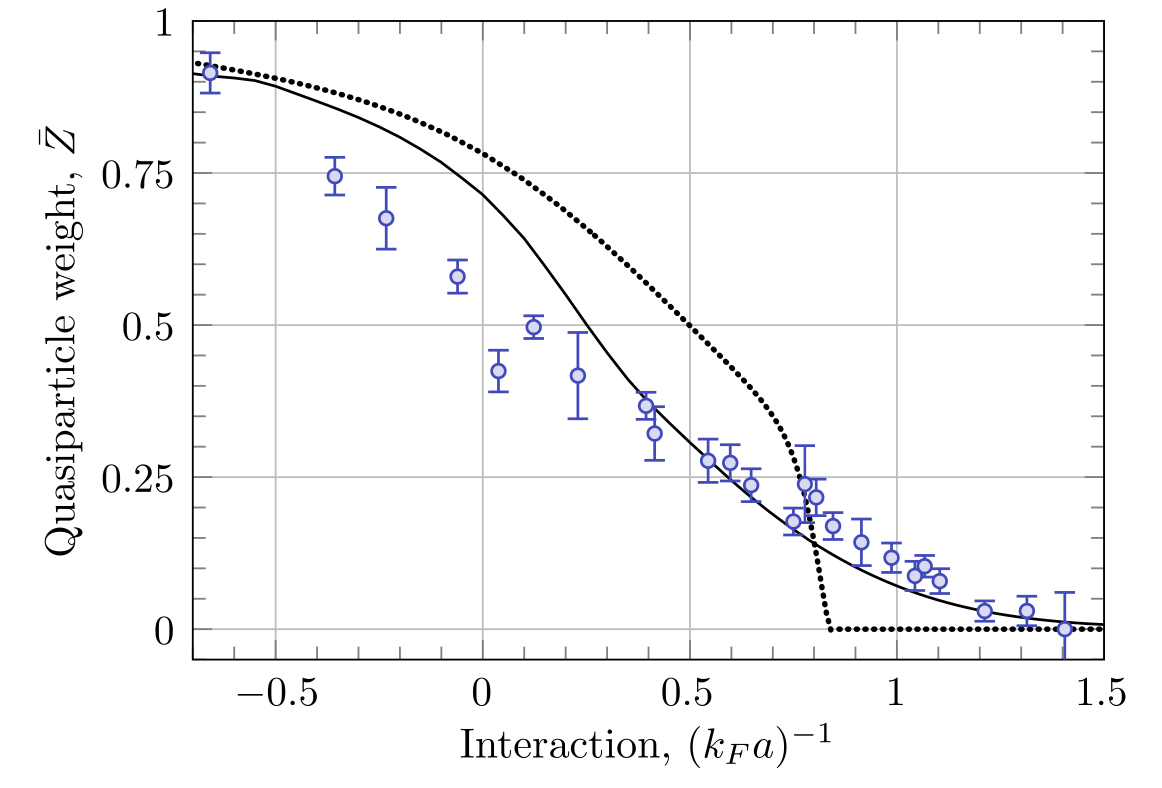
\includegraphics[width=0.7\textwidth]{./intro/chap1smooth.png}
    \bicaption{Raman谱实验得到的平均准粒子剩余$Z$。其中散点代表实验观测数据,实线代表LDA近似的结果,点线代表单杂质在$T
    =0$下的准粒子剩余。摘自\citep{Sagi2020}}{Quasiparticle residue obtained from fitting Raman Spectrum. Scattered points for experiment results, solid line for LDA results and dotted line for single impurity results at $T=0$. Reprinted from\citep{Sagi2020}}
    \label{fpsmooth}
\end{figure}
%%%%%%%%%%%%%%%%%%%%%%%%%%%%%%%%%%%%%%%%%%%%%%%%%%%%%%%%%%%%%%%%%%%%%%%%%%




\section{本征热化假说}\label{1sec:ETH}
热化一直是统计物理中很基础的概念。统计物理中(经典或者量子)宏观数目自由度体系在到达热力学平衡态之后,体系热力学性质可以仅用几个参数来描述(如温度、压强、化学势等),宏观可观测量由热力学统计分布给出。为什么宏观体系可以仅用几个参数来描述?宏观体系是如何到达热力学平衡态的?如何在量子力学的层面去理解这一热化现象?基于这些非常基本的问题,用来理解量子系统热化现象的假说——本征热化假说被提出。我们在这一节中详细介绍一下目前的研究进展。更加详细的讨论参见\cite{d2016quantum,deutsch2018eigenstate}。

一个孤立体系的量子力学的演化是幺正的,从初态出发,初态在不同本征态上的权重是不随时间变化的。但是最终随着长时间的演化,系统的宏观可观测量不依赖于初态的权重分布。仅有几个参数所确定。此时一个自然的想法被提出来———本征热化假说\cite{Deutsch1991quantum,Srednicki1994chaos,srednicki1999approach}。其核心思想为对于能量处于$\bar{E}=\langle\psi_I|\hat{H}|\psi_I\rangle$附近的本征态,其局域算符的平均值是一样的。我们用形式化的语言来表述,考虑一个孤立系统$\hat{H}$,本征态于本征能量:$\hat{H}|m\rangle=E_m|m\rangle$。从任意初态出发时间演化得到t时刻波函数:
\begin{equation}
|\psi(t)\rangle=\sum_{m} C_{m} \mathrm{e}^{-i E_{m} t}|m\rangle
\end{equation}
其中$C_m = \langle m | \psi_I\rangle$,出于方便我们取$\hbar=1$。对某个局域算符可观测量$\hat{O}$来说,t时刻观测期望值为:
\begin{equation}
\begin{aligned}
O(t) & \equiv\langle\psi(t)|\hat{O}| \psi(t)\rangle=\sum_{m, n} C_{m}^{*} C_{n} e^{i\left(E_{m}-E_{n}\right) t} O_{m n} \\
&=\sum_{m}\left|C_{m}\right|^{2} O_{m m}+\sum_{m, n \neq m} C_{m}^{*} C_{n} e^{i\left(E_{m}-E_{n}\right) t} O_{m n}
\end{aligned}
\end{equation}
其中$O_{m n}=\langle m|\hat{O}| n\rangle$。如果体系最终热化,则局域算符的长时间平均应该等于微正则系综平均,并且$O(t)$的长时间行为应该围绕这一平均值做热力学涨落。此时根据本征热化假说,对于热化的体系,$O_{mn}$满足:
\begin{equation}
O_{m n}=O(\bar{E}) \delta_{m n}+e^{-S(\bar{E}) / 2} f_{O}(\bar{E}, \omega) R_{m n}
\end{equation}
其中$\bar{E} \equiv\left(E_{m}+E_{n}\right) / 2, \omega \equiv E_{n}-E_{m}$。$S(E)$是能量为E时候的热力学熵。$O(\bar{E})$与$f_{O}(\bar{E}, \omega)$为光滑单值函数。$R_{m n}$为随机变量,满足$\overline{\left|R_{m n}\right|^{2}}=1$。这一假设目前没有严格的证明。但是有很多数值上的验证。其中对角元部分与长时间平均值有关,非对角元部分则与围绕平均值的涨落有关。考虑$O(t)$的长时间平均,在这里我们考虑广义的封闭系统,将对称性考虑进去之后,系统没有简并,这个假设是合理的,因此:
\begin{equation}
\bar{O} \equiv \lim _{t_{0} \rightarrow \infty} \frac{1}{t_{0}} \int_{0}^{t_{0}} d t O(t)=\sum_{m}\left|C_{m}\right|^{2} O_{m m}=\operatorname{Tr}\left[\hat{\rho}_{\mathrm{DE}} \hat{O}\right]
\end{equation}
其中$\hat{\rho}_{DE}$为对角系综。我们定义初态的能量方差为:
\begin{equation}
\delta E \equiv \sqrt{\left\langle\psi_{I}\left|\hat{H}^{2}\right| \psi_{I}\right\rangle-\left\langle\psi_{I}|\hat{H}| \psi_{I}\right\rangle^{2}}
\end{equation}
如果方差很小,那么就会有:
\begin{equation}
\bar{O} \simeq O(\langle E\rangle) \simeq O_{\mathrm{ME}}
\end{equation}
进一步,我们量化这一差异,考虑泰勒展开:
\begin{equation}
O_{m m} \approx O(\langle E\rangle)+\left.\left(E_{m}-\langle E\rangle\right) \frac{d O}{d E}\right|_{\langle E\rangle}+\left.\frac{1}{2}\left(E_{m}-\langle E\rangle\right)^{2} \frac{d^{2} O}{d E^{2}}\right|_{\langle E\rangle}
\end{equation}
将其带入长时间平均得到:
\begin{equation}
\bar{O} \approx O(\langle E\rangle)+\frac{1}{2}(\delta E)^{2} O^{\prime \prime}(\langle E\rangle) \approx O_{\mathrm{ME}}+\frac{1}{2}\left[(\delta E)^{2}-\left(\delta E_{\mathrm{ME}}\right)^{2}\right] O^{\prime \prime}(\langle E\rangle)
\end{equation}
其中$\delta_{ME}$为微正则系综的能量涨落标准差。而对于仅有局域相互作用的孤立系统来说$\delta E$为:
\begin{equation}
\begin{array}{r}
\delta E \equiv \sqrt{\langle\psi_{I}|\hat{H}^{2}| \psi_{I}\rangle-\langle\psi_{I}|\hat{H}| \psi_{I}\rangle^{2}}=\sqrt{\langle\psi_{I}|\hat{H}_{1}^{2}| \psi_{I}\rangle-\langle\psi_{I}|\hat{H}_{1}| \psi_{I}\rangle^{2}} \\
=\sqrt{\sum_{j_{1}, j_{2}}\left[\langle\psi_{I}|\hat{h}_{j_{1}} \hat{h}_{j_{2}}| \psi_{I}\rangle-\langle\psi_{I}|\hat{h}_{j_{1}}| \psi_{I}\rangle\langle\psi_{I}|\hat{h}_{j_{2}}| \psi_{I}\rangle\right]}
\end{array}
\end{equation}
其中$\hat{H}=\hat{H}_{0}+\hat{H}_{1}$,$\hat{H}_{1}=\sum_{j} \hat{h}_{j}$仅有局域关联的算符。因此通常情况下有:
\begin{equation}
\delta E \sim \sqrt{V}
\end{equation}
继而有$\delta E / E \sim 1 / \sqrt{V}$。因此这一差异在热力学极限下趋近于0。

我们然后计算局域算符平方的长时间涨落:
\begin{equation}
\begin{aligned}
\sigma_{O}^{2} & \equiv \lim _{t_{0} \rightarrow \infty} \frac{1}{t_{0}} \int_{0}^{t_{0}} d t[O(t)]^{2}-(\bar{O})^{2} \\
&=\lim _{t_{0} \rightarrow \infty} \frac{1}{t_{0}} \int_{0}^{t_{0}} d t \sum_{m, n, p, q} O_{m n} O_{p q} C_{m}^{*} C_{n} C_{p}^{*} C_{q} \mathrm{e}^{i\left(E_{m}-E_{n}+E_{p}-E_{q}\right) t}-(\bar{O})^{2} \\
&=\sum_{m, n \neq m}\left|C_{m}\right|^{2}\left|C_{n}\right|^{2}\left|O_{m n}\right|^{2} \leq \max \left|O_{m n}\right|^{2} \sum_{m, n}\left|C_{m}\right|^{2}\left|C_{n}\right|^{2}=\max \left|O_{m n}\right|^{2} \propto \exp [-S(\bar{E})]
\end{aligned}
\end{equation}
可以看到这一涨落由非对角元控制,且随系统体积被指数压低。我们接着去看局域算符涨落的方差:
\begin{equation}
\overline{\delta O^{2}}=\lim _{t_{0} \rightarrow \infty} \frac{1}{t_{0}} \int_{0}^{t_{0}} d t\left\langle\psi(t)\left|(\hat{O}-\bar{O})^{2}\right| \psi(t)\right\rangle=\sum_{m}\left|C_{m}\right|^{2}\left(O^{2}\right)_{m m}-\bar{O}^{2}
\end{equation}
同样也有:
\begin{equation}
\sqrt{\overline{\delta O^{2}}} / \bar{O} \simeq \sqrt{\delta O_{\mathrm{ME}}^{2}} / O_{\mathrm{ME}} \simeq 1 / \sqrt{V}
\end{equation}
由以上分析,我们可以理解,在本征热化假设成立的前提下,孤立系统局域算符的长时间平均等于热力学吉布斯平均(包括微正则、正则与巨正则系综)。那么本征热化假设有哪些成立的证据呢?目前来讲证据主要来自于格点系统的数值模拟。主要的模型包括硬核玻色子模型\cite{rigol2008thermalization,Santos2010Localization,Rigol2009Breakdown,Rigol2010Quantum,Neuenhahn2012Thermalization,Steinigeweg2013Eigenstate,Kim2014testing,beugeling2014finite,Steinigeweg2014Pushing,Khodja2015Relevance,Beugeling2015Off-diagonal}以及横场伊辛模型\cite{Fratus2015Eigenstate,Mondaini2016Eigenstate,Mondaini2017Eigenstate,blass2016test,Serbyn2013local}。我们挑选其中有代表性工作介绍,如图~\ref{ETHnum}~所示,展示了一维硬核玻色子与带纵场的横场伊辛模型的数值结果\cite{Kim2014testing}。可以看到对角元部分随着系统尺寸的增大局域算符的本征态期望值逐渐收敛到与能量有关的单值函数。
%%%%%%%%%%%%%%%%%%%%%%%%%%%%%%%%%%%%%%%%%%%%%%%%%%%%%%%%%%%%%%%%%%%%%%%%%%
\begin{figure}[!htbp]
    \centering
    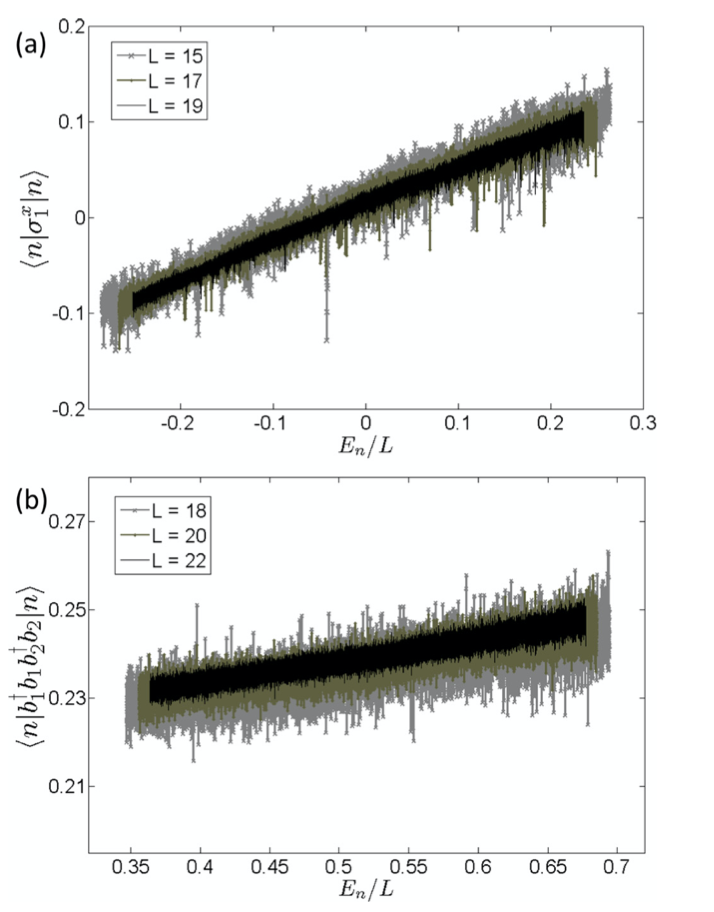
\includegraphics[width=0.7\textwidth]{./intro/chap1ETHnum.png}
    \bicaption{局域算符的对角元随本征能量的分布。其中(a)为带纵场的横场伊辛模型。(b)为带有次近邻相互作用的硬核玻色子模型。 摘自\citep{Kim2014testing}}{Eigenstate expectation value of local operators vs eigen energy. Fig (a) for TFIM with longitudinal filed and Fig (b) for hard core bosons with next-nearest-neighbor interaction. Reprinted from\citep{Kim2014testing}}
    \label{ETHnum}
\end{figure}
%%%%%%%%%%%%%%%%%%%%%%%%%%%%%%%%%%%%%%%%%%%%%%%%%%%%%%%%%%%%%%%%%%%%%%%%%%
而对于非对角元部分的验证也有部分数值验证,不过还尚未成熟,可以参见\cite{Beugeling2015Off-diagonal,Mondaini2017Eigenstate}。

本征热化假说(ETH)本身以及其数值证据,吸引着越来越多研究者的注意。但这一假说是个要求很强的假说。随着研究者对此认识的不断加深,越来越多的违背本征热化假说的系统被发现。其中以量子可积系统\cite{kinoshita2006quantum,Rigol2007Relaxation,Calabrese2011Quantum,essler2016quench,vidmar2016generalized}与多体局域化系统\cite{basko2006metal,Serbyn2013local,Huse2014Phenomenology}最为典型,这两种体系是完全的本征热化假说破缺的体系,并且得到了实验的验证。


除了这种完全违背本征热化假说的系统,随着实验手段的进步,最近在实验中发现了弱违背本征热化假说的体系,其中以量子多体伤痕为典型例子。量子多体伤痕最早来源于里德堡原子的实验,在51个原子的一维链中,观测到$|Z_2\rangle$初态出发的反常动力学,其长时间震荡行为与长时间平均值均表明非热化的发生\cite{bernien2017probing}。如图所示~\ref{scar}~。
%%%%%%%%%%%%%%%%%%%%%%%%%%%%%%%%%%%%%%%%%%%%%%%%%%%%%%%%%%%%%%%%%%%%%%%%%%
\begin{figure}[!htbp]
    \centering
    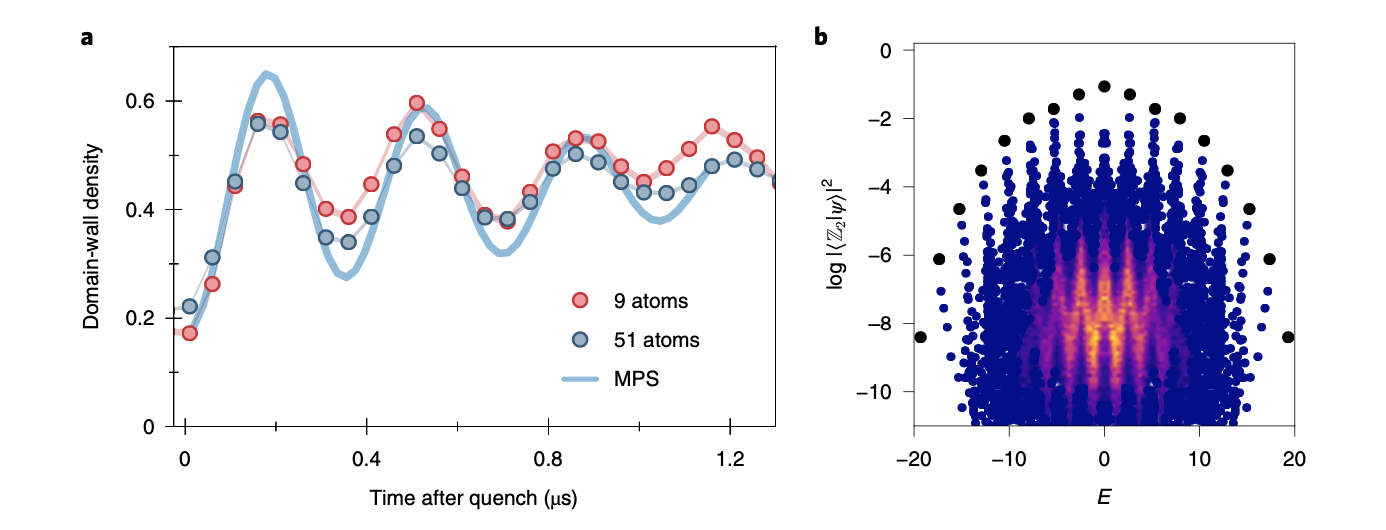
\includegraphics[width=0.7\textwidth]{./intro/chap1scar.png}
    \bicaption{多体伤痕物理。图a为里德堡实验平台观察到的量子多体伤痕动力学,图b为后续通过与$|Z_2\rangle$做投影筛选得到非热化子空间。摘自\citep{bernien2017probing,serbyn2021quantum}}{Many body scars physics. Fig a for many body scar dynamics from Rydberg atoms simulation and Fig b for non-thermalized sub Hilbert space obtained from overlap with $|Z_2\rangle$. Reprinted from\citep{bernien2017probing,serbyn2021quantum}}
    \label{scar}
\end{figure}
%%%%%%%%%%%%%%%%%%%%%%%%%%%%%%%%%%%%%%%%%%%%%%%%%%%%%%%%%%%%%%%%%%%%%%%%%%
对这一实验的理论研究表明,反常动力学存在的原因为本征态希尔伯特空间中近似分立的子空间,其维度正比于链长。这一子空间在可以通过与初态$|Z_2\rangle$做投影,或者计算局域算符的本征态期望值,或者计算本征态的半链纠缠熵挑选出来\cite{turner2018weak,Turner2018quantum,Ho2019periodic,Choi2019emergent,Michailidis2020slow,serbyn2021quantum},如图~\ref{scar}~所示。

围绕着本征热化假说,孤立体系的热化的神秘面纱被逐步揭开。伴随着量子模拟实验技术的进步,我们对于热化的了解也会越来越深入下去,但是同样的未知也在逐步增多,这仍是一个在蓬勃发展的领域。





\section{本文安排}\label{1sec:sum}
在接下来的章节中,我们首先在第~\ref{chap:kondo}~章中从相对简单的少体磁性杂质体系出发,考虑一维下局域自旋与两个巡游费米子之间在自旋交换相互作用影响下的能谱结构,揭示少体体系的基态与激发态中蕴藏的特殊少体关联行为。然后转入第~\ref{chap:polaron}~章,我们从少体杂质体系来到多体杂质的研究。我们考虑典型的费米极化子物理,采用统一的变分波函数研究基态从极化子到分子的转变,揭示这一转变的本质在于基态从零动量到费米动量的转移,讨论维度与泡利禁闭机制在这一转变中发挥的作用。并且基于转变点附近的极化子与分子共存机制讨论了实验体系中有限温度和有限密度对单粒子观测量的连续化影响。在第~\ref{chap:ETH}~章我们从能谱的静态行为转变到动力学行为研究,系统地考察带有纵场的横场伊辛模型中,从固定初态出发,选取不同的耦合参数计算局域算符的时间平均与热力学系综平均得到热化的相图。在第~\ref{chap:sum}~章总结并展望这一从少体到多体再到动力学的研究脉络,这有助于我们对量子体系新奇物理特性理解的深入。


